%% 
%% Copyright 2007-2024 Elsevier Ltd
%% 
%% This file is part of the 'Elsarticle Bundle'.
%% ---------------------------------------------
%% 
%% It may be distributed under the conditions of the LaTeX Project Public
%% License, either version 1.3 of this license or (at your option) any
%% later version.  The latest version of this license is in
%%    http://www.latex-project.org/lppl.txt
%% and version 1.3 or later is part of all distributions of LaTeX
%% version 1999/12/01 or later.
%% 
%% The list of all files belonging to the 'Elsarticle Bundle' is
%% given in the file `manifest.txt'.
%% 
%% Template article for Elsevier's document class `elsarticle'
%% with harvard style bibliographic references

\documentclass[preprint,12pt]{elsarticle}

%% Use the option review to obtain double line spacing
%% \documentclass[authoryear,preprint,review,12pt]{elsarticle}

%% Use the options 1p,twocolumn; 3p; 3p,twocolumn; 5p; or 5p,twocolumn
%% for a journal layout:
%% \documentclass[final,1p,times,authoryear]{elsarticle}
%% \documentclass[final,1p,times,twocolumn,authoryear]{elsarticle}
%% \documentclass[final,3p,times,authoryear]{elsarticle}
%% \documentclass[final,3p,times,twocolumn,authoryear]{elsarticle}
%% \documentclass[final,5p,times,authoryear]{elsarticle}
%% \documentclass[final,5p,times,twocolumn,authoryear]{elsarticle}

%% For including figures, graphicx.sty has been loaded in
%% elsarticle.cls. If you prefer to use the old commands
%% please give \usepackage{epsfig}

%% The amssymb package provides various useful mathematical symbols
\usepackage{amssymb}
%% The amsmath package provides various useful equation environments.
\usepackage{amsmath}
%% The amsthm package provides extended theorem environments
%% \usepackage{amsthm}
\usepackage{comment} 
\usepackage{color}
\usepackage{url}
\usepackage{subcaption}
\usepackage{algorithm}
\usepackage{algpseudocode} % o algorithmicx
%% The lineno packages adds line numbers. Start line numbering with
%% \begin{linenumbers}, end it with \end{linenumbers}. Or switch it on
%% for the whole article with \linenumbers.
%% \usepackage{lineno}

\journal{Remote Sensing Applications: Society and Environment}

\begin{document}

\begin{frontmatter}

%% Title, authors and addresses

%% use the tnoteref command within \title for footnotes;
%% use the tnotetext command for theassociated footnote;
%% use the fnref command within \author or \affiliation for footnotes;
%% use the fntext command for theassociated footnote;
%% use the corref command within \author for corresponding author footnotes;
%% use the cortext command for theassociated footnote;
%% use the ead command for the email address,
%% and the form \ead[url] for the home page:
%% \title{Title\tnoteref{label1}}
%% \tnotetext[label1]{}
%% \author{Name\corref{cor1}\fnref{label2}}
%% \ead{email address}
%% \ead[url]{home page}
%% \fntext[label2]{}
%% \cortext[cor1]{}
%% \affiliation{organization={},
%%            addressline={}, 
%%            city={},
%%            postcode={}, 
%%            state={},
%%            country={}}
%% \fntext[label3]{}

\title{MAPunet: High-Resolution Snow Depth Mapping through U-Net Pixel-wise Regression}

%% use optional labels to link authors explicitly to addresses:
%% \author[label1,label2]{}
%% \affiliation[label1]{organization={},
%%             addressline={},
%%             city={},
%%             postcode={},
%%             state={},
%%             country={}}
%%
%% \affiliation[label2]{organization={},
%%             addressline={},
%%             city={},
%%             postcode={},
%%             state={},
%%             country={}}

\author[label1]{Alejandro Betato}
\ead{abetatos@gmail.com}
\author[label2]{Hernán Díaz Rodríguez}
\ead{diazhernan@uniovi.es}
\author[label3]{Niamh French}
\ead{niamh.french@wegaw.com}
\author[label3]{Thomas James}
\ead{thomas.james@wegaw.com}
\author[label2]{Beatriz Remeseiro\corref{cor1}}


\affiliation[label1]{organization={Menendez Pelayo International University}, country={Spain}}

\affiliation[label2]{organization={Department of Computer Science, University of Oviedo}, country={Spain}}

\affiliation[label3]{organization={AI \& Earth Observation, Wegaw}, country={Switzerland}}

\cortext[cor1]{Corresponding author. Email: bremeseiro@uniovi.es}

%% Abstract
\begin{abstract}
%% Text of abstract
Accurate snow depth prediction is essential for hydrological risk assessment, flood prediction, water resource management, and weather forecasting. While previous studies have successfully applied deep learning techniques to generate snow depth maps, many have been constrained by geographical coverage or low data resolution. This work addresses these limitations by integrating high-resolution LiDAR maps, satellite imagery, digital elevation models, and three novel time-dependent variables. Additionally, the well-known U-Net architecture has been customized to perform pixel-wise regression and accurately predict snow depth over large geographic areas. The proposed method, called MAPunet, effectively models snow depth in the mountainous region of Davos, achieving an average error of 0.62 m at a 5 m resolution. The experimental results demonstrate the potential of combining high-resolution data with advanced deep learning techniques for enhanced snow depth mapping.
\end{abstract}

%%Graphical abstract
%%\begin{graphicalabstract}
%\includegraphics{grabs}
%%\end{graphicalabstract}

%%Research highlights
\begin{highlights}
\item A refined U-Net architecture for precise pixel-wise regression over large areas.
\item Feature engineering from high-resolution LiDAR maps and digital elevation models.
\item Three novel time-dependent variables for better snow depth prediction.
\item Competitive results with an average error of 0.52 m at a resolution of 5 m in Davos.
\end{highlights}

%% Keywords
\begin{keyword}
%% keywords here, in the form: keyword \sep keyword
Pixel-wise Regression \sep Snow Depth Maps \sep High-Resolution Data
%% PACS codes here, in the form: \PACS code \sep code

%% MSC codes here, in the form: \MSC code \sep code
%% or \MSC[2008] code \sep code (2000 is the default)

\end{keyword}

\end{frontmatter}

%% Add \usepackage{lineno} before \begin{document} and uncomment 
%% following line to enable line numbers
%% \linenumbers

%% main text
%%
\section{Introduction}
\label{Sec:introduction}

High Alpine regions show great potential for solar photovoltaic electricity production in winter due to the reflective properties of snow \cite{xu2013snow} and the larger number of hours of sunlight compared to the lower urban and peri-urban regions \cite{fenrg.2024}. Within this context, in Alpine environments, the chosen height for solar panel installation affects their performance and energy generation capacity: while increased albedo and forward scattering can enhance energy yields \cite{vonRtte2021}, snow accumulation can significantly reduce performance through panel coverage or burial. The relationship between height and performance becomes apparent when considering that raising panels by just one meter can reduce snow coverage by up to 100 days annually, resulting in longer operational periods for the facility \cite{wegawSuperResolutionSnow}. Additionally, accurate snow depth predictions are essential for various applications, such as forecasting and managing water resources, particularly in rugged mountain landscapes where snow contributes significantly to the formation of seasonal water reserves \cite{dewalle2008principles}.

Our research work aims to develop a high-resolution model for mapping peak season snow depth in the Davos region of Eastern Switzerland, while exploring the potential for extending these predictions to other locations. The model is designed to provide data-driven guidance for solar panel positioning height above snow level. Additionally, we investigate both static and dynamic variables that could serve as meaningful predictors for these estimations. The study is conducted in collaboration with the geospatial company Wegaw\footnote{https://wegaw.com/}, specialized in commercialization of data for snow and water digital twins. The selection of Davos as our primary study area is driven by the availability of comprehensive input datasets, including diverse training maps and multiple measurement stations, and the presence of potential solar energy stakeholders interested in panel installations given that placing photovoltaic installations in alpine areas can increase the market value of the produced electricity between 25\% and 33\%~\cite{Kahl2019,Dujardin2022}. 

Remote sensing techniques have emerged as valuable tools for measuring snow depth in challenging terrains, offering solutions to the limitations of ground-based methods. To overcome these challenges, Liu et al. \cite{liu2019retrieval} employed brightness temperature data from passive microwave radiometers to estimate snow depth over the Arctic Ocean at a spatial resolution of 25 km. However, passive microwave snow depth measurements are often unreliable in mountainous terrain due to saturation at higher snow depths and insufficient spatial resolution to capture snow depth variability at the kilometer scale, presenting substantial challenges \cite{Tedesco2010, Tong2010, Smith2018}. %Tanniru2023

Airborne Laser Imaging Detection and Ranging (LiDAR) is one of the most reliable methods for mapping snow depth providing, spatial resolutions finer than one meter and errors below one decimeter \cite{revuelto2021intercomparison, deems2013lidar, buhler2016mapping}. Its precise mapping capabilities have made LiDAR imagery an invaluable tool for higher-resolution snow modeling. Wulf et al. \cite{wulf2020high} validated a snow depth prediction approach using snow depth measurements from flights over the European Alps and the Rocky Mountains. Cartwright et al. \cite{cartwright2022machine} utilized LiDAR imagery to train a snow depth prediction model in southwestern Alberta, while Dharmadasa et al. \cite{Dharmadasa2023, Dharmadasa2024} applied LiDAR to characterize snow depth distribution in agroforestry environments in Quebec, Canada. However, the high costs associated with LiDAR acquisition have limited the availability of publicly accessible snow depth maps derived from this technology. 

Machine learning (ML) approaches have become prominent in snow hydrology due to their capability to model complex, non-linear snow processes that are challenging to represent with traditional techniques. Classical ML approaches for snow depth modeling include regression trees \cite{winstral2002spatial}, random forest regression \cite{hu2021snow}, and support vector regression \cite{hu2021snow}, while deep learning approaches have also been explored, including deep belief networks \cite{wang2020estimating} or recurrent networks \cite{meyal2020automated}. Convolutional neural networks (CNNs) have gained particular attention, as demonstrated by Xing et al. \cite{xing2022estimation}, who proposed a deep residual network for snow depth prediction at a 25 km resolution.

% To the best of our knowledge, only a few research works have addressed the challenge of snow modeling with ML} at high spatial resolution. 
High-resolution snow depth modeling with ML is an emerging research area. While Geissler et al. \cite{Geissler2023} achieved high accuracy with a root mean square error (RMSE) between 0.09 and 0.11 m at 1 m$^2$ resolution, their study was limited to a small sub-alpine area of 0.3 km$^2$ with moderate slopes. Similarly, Revuelto et al. \cite{revuelto2020random} applied Random Forest algorithms to three sites totaling 1.03 km², but their approach showed limitations when applied to locations not included in the training dataset. Daudt et al. \cite{daudt2023snow} utilized a ConvGRU cell-based CNN to achieve 10 m resolution snow depth predictions, with an RMSE of 0.44--0.92 m through a recurrent approach that incorporates previous temporal data. However, their method does not leverage meteorological station data, a key source for snow depth variability. % achieved a root mean square error (RMSE) of 0.44-0.92 m at 10 m resolution using  \cite{ballas2015delving}. They proposed a recurrent approach that allows the model to sample the previous days to predict the following one.

Satellite data provide an avenue for high-resolution snow depth mapping, offering broad spatial coverage and frequent revisits. In recent years, satellite imagery has become more accessible to the general public through missions such as Copernicus\footnote{\url{https://www.copernicus.eu}} of the European Space Agency (ESA) or MODIS\footnote{\url{https://modis.gsfc.nasa.gov}} of the American National Aeronautics and Space Administration (NASA). The analysis by Eberhard et al. \cite{eberhard2021intercomparison} revealed that snow depth maps generated from satellite imagery with approximately 10 m resolution achieved an RMSE ranging from 0.5 to 1.0 m. Similarly, Dunmire et al. \cite{dunmire2024machine} and Broxton et al. \cite{broxton2024improving} employed ML methods for SAR-based snow depth mapping at 100 m and 500 m resolutions, respectively, improving upon traditional models in capturing topography-driven snow variability. % introduce a machine learning approach to improve SAR-based snow depth estimation at 100 m resolution, enhancing local-scale topography-driven variability over the European Alps. Broxton et al. evaluate Sentinel-1 SAR snow depth data against airborne datasets over the Colorado Rockies and Sierra Nevada applying machine learning to improve accuracy and produce complete snow depth maps with 500 m resolution \cite{broxton2024improving}.

Encoder-decoder architectures, such as U-Net \cite{ronneberger2015u} and its variants, are widely used in hydrological modeling with satellite imagery. These architectures are neural networks trained to encode input data into a lower-dimensional representation and then decode it back to its original dimensions. In this context, Yao et al. \cite{YAO2018} applied U-Net for pixel-wise regression in pan-sharpening, while Taccari et al. \cite{TACCARI2022} explored an attention U-Net model for groundwater level prediction. % introduced a pixel-wise regression approach utilizing the U-Net architecture for pan-sharpening. For their part,} Taccari et al. \cite{TACCARI2022} explored the application of the attention U-Net model in predicting groundwater levels. 
% Taccari et al. \cite{TACCARI2022} explored the application of the attention U-Net model in predicting groundwater levels, while Rasiya Koya et al. \cite{RasiyaKoya2023} proposed an autoencoder-based snow drought index. Different versions of U-Net architecture \cite{Sudakow2022, Sultana2023} have also been used for the detection of melt ponds on the arctic sea ice through high-resolution aerial photographs, or to build surrogate models performing with limited datasets \cite{WANG2021, Zhu2018}.
Other U-Net adaptations have been applied in various hydrological contexts, including snow detection \cite{Yin2022, Wang2022, Ma2023}. However, these models generally do not integrate additional variables beyond satellite data, such as meteorological station measurements or terrain features, limiting their effectiveness in snow depth modeling.
% Regarding snow detection, Yin et al. \cite{Yin2022} proposed an improved Unet3+ to extract clouds and snow from remote sensing images. Wang et al. \cite{Wang2022} investigated snow coverage mapping by learning from Sentinel-2 satellite multispectral images, proving that U-Net can outperform other deep learning methods. For their part, Ma et al. \cite{Ma2023} proposed a UCTNet with dual-flow architecture to process snow coverage mapping with Sentinel-2 satellite imagery. To the extent of our knowledge, none of these proposals incorporate variables other than satellite images, such as dynamic ground measurements or specific characteristics of a geographical region, like elevation or slope.

% Faced with the challenges of accurately predicting snow depth, crucial for environmental and hydrological analyses, this research work presents a novel approach to improve snow depth mapping. In particular, we propose 
To address these limitations, our work proposes a custom U-Net architecture designed for pixel-wise regression that generates high-resolution snow depth maps from satellite imagery. The main contributions of our work are:

\begin{itemize}
\item \textbf{Feature analysis and selection.} Identification and selection of the most informative features for 5 m resolution snow depth estimation. % We have identified and analyzed the informativeness of ten input features, and selected the most appropriate dataset for snow depth estimation at a 5m spatial resolution.

\item \textbf{Temporal variability.} Development of three novel methods to incorporate temporal data from meteorological stations, enhancing predictive accuracy. %We have devised three novel methods to incorporate temporal variability into our analysis, using data from meteorological stations collected over time. 
% It has been demonstrated that the more accurate these variables are, the more accurate the predictions.

\item \textbf{MAPunet architecture.} Introduction of MAPunet, an optimized U-Net adaptation for detailed, pixel-wise snow depth prediction. % We introduce MAPunet, an innovative adaptation of the U-Net architecture \cite{ronneberger2015u}, specifically customized for pixel-wise regression to generate detailed snow depth maps.

\item \textbf{MAPchete generator.} A novel image generation technique that standardizes spatial representations for data augmentation. % We present MAPchete \cite{mapCHETE}, a unique image generation technique that transforms irregular maps into standardized square images. This approach not only ensures a uniform representation of each area within the dataset but also acts as an effective method for data augmentation.
\end{itemize}

The remainder of the manuscript is organized as follows. Section \ref{Sec:Features} describes the selected variables, Section \ref{Sec:Methodology} presents the MAPunet architecture and the MAPchete generator, Section \ref{Sec:ExperimentalSetup} outlines the reference data and the experimental setup, Section \ref{Sec:Results} provides a variable analysis and an ablation study to identify the most informative features, and Section \ref{Sec:discussion} concludes with findings and future research directions.

\section{Feature description} \label{Sec:Features}

Snow depth is affected by a wide variety of physical processes. To encapsulate this complexity, we propose a set of representative features computed from the Digital Elevation Model (DEM) and Wegaw Snow Cover Extent (SCE) maps. Specifically, we have selected variables recently identified in the literature as crucial for accurate snow depth estimation. Moreover, we have enriched our analysis by incorporating temporal variability, utilizing data collected over time from meteorological stations. All variables have been normalized to the range $[0,1]$, ensuring comparability across different scales. These variables are illustrated in Fig. \ref{fig:Variables} and detailed below.

\begin{figure}[htbp]
    \centering
    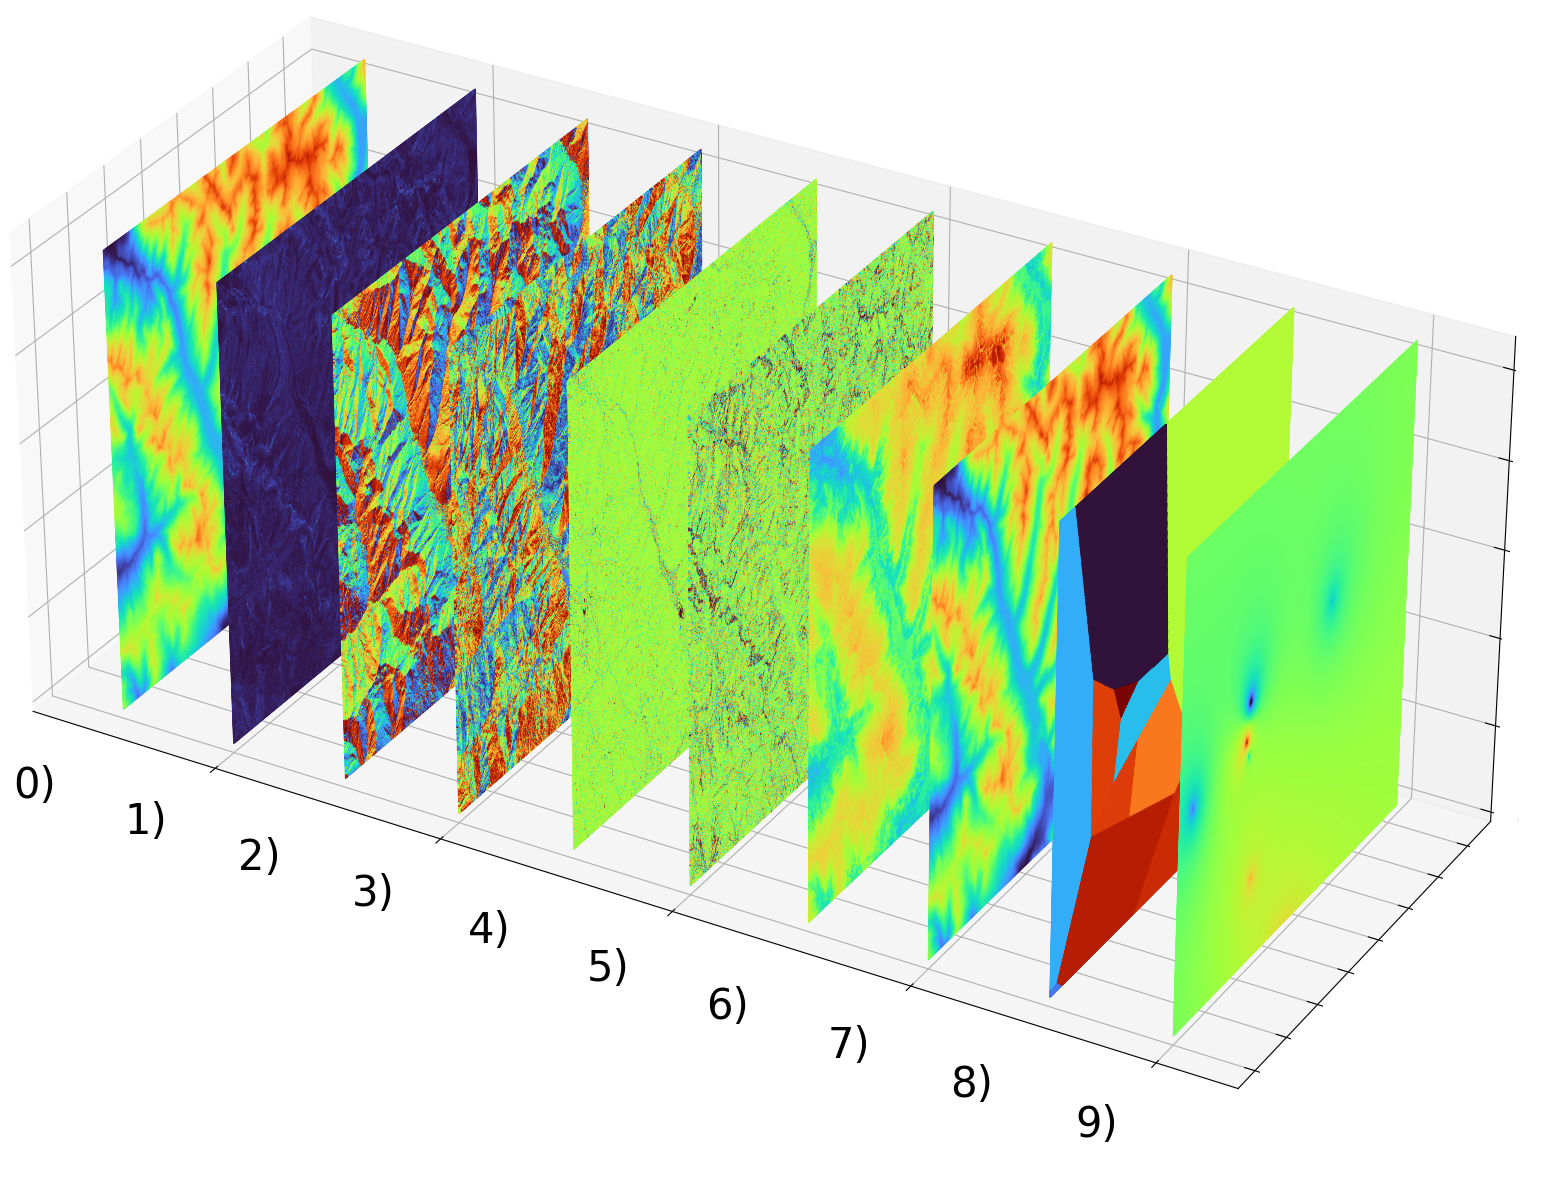
\includegraphics[width=0.7\columnwidth]{Variables.png}
    \caption{Representative sample of the ten input variables considered: 0) DEM, 1) Slope, 2) Aspect, 3) FFD, 4) TPI, 5) TPI-Alt, 6) SCE, 7) DEMStat, 8) Voronoi, and 9) ProbStat. The values have been normalized to $[0, 1]$, with the color scale representing the lowest values in blue and the highest values in red.}
    \label{fig:Variables}
\end{figure}


\subsection{Digital elevation models}

A digital elevation model (DEM) is a two-dimensional matrix in which each value represents the elevation, providing an understanding of the spatial characteristics of the environment. DEM models for Switzerland are publicly available from the Federal Office of Topography\footnote{\url{https://www.swisstopo.admin.ch/en/geodata/height/alti3d.html}}. They consist of a three-dimensional representation of the Swiss Alps with a spatial resolution of 0.5 m.

\subsection{Slope}

The slope of a surface is, by definition, the derivative of its elevation. The usefulness of this variable lies in the fact that snow tends to accumulate more in flat areas while it tends to diminish in steeper ones. Additionally, the slope plays a role in the amount of radiative energy the surface receives \cite{zhu2021downscaling}.

\subsection{Surface aspect}
\label{subsec:aspect}

The surface aspect represents the angle between the surface normal and the North vector $\Vec{D}$. For instance, an angle of $0^\circ$ depicts a slope facing north, whereas $90^\circ$ represents a slope facing east. It has been demonstrated to be an effective variable when modeling snow depth, as surfaces facing the same direction exhibit similar exposure to external factors \cite{zhong2021impacts}. 

\subsection{Far from $\Vec{D}$}
\label{subsec:ffd}

In this section, we introduce a segmented snow analysis methodology that facilitates a systematic examination of snow-terrain relationships by dividing measurements into discrete intervals. Based on this, we develop the Far From $\Vec{D}$ (FFD) metric, which measures the angular distance between surface aspects and the direction of minimum snow accumulation. Together, these analyses reveal patterns in snow depth distribution and their correlation with terrain orientation.

\subsubsection{Segmented Snow Analysis}

Segmented snow analysis provides a systematic approach to examining snow depth distribution across topographical features by dividing snow depth measurements into discrete intervals based on elevation. % a given topographical parameter, enabling a more structured examination of snow-terrain relationships.
Figure \ref{fig:slicing} illustrates this approach: Figure \ref{fig:slicinga} shows the raw data distribution of snow depth versus elevation in the Davos region, while Figure \ref{fig:slicingb} displays the segmented data, averaged at 1 m elevation intervals, revealing a clearer relationship between snow depth and elevation. %The relationship between snow depth and elevation becomes more distinct after implementing this segmentation methodology.}

\begin{figure*}[htbp]
  \begin{subfigure}{0.49\textwidth}
    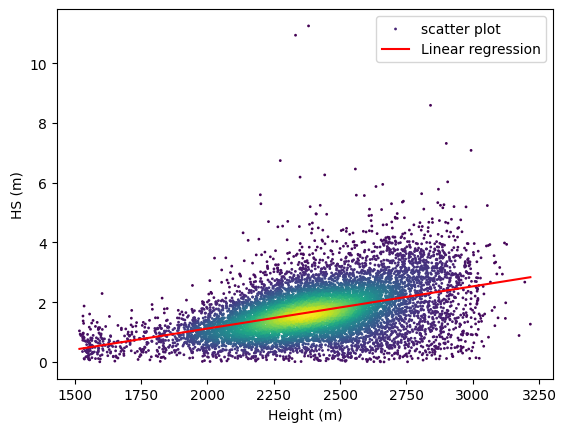
\includegraphics[width=\textwidth]{Slicing_before.png}
      \caption[Image 1]{}
      \label{fig:slicinga}
  \end{subfigure}
  \hfill
  \begin{subfigure}{0.49\textwidth}
    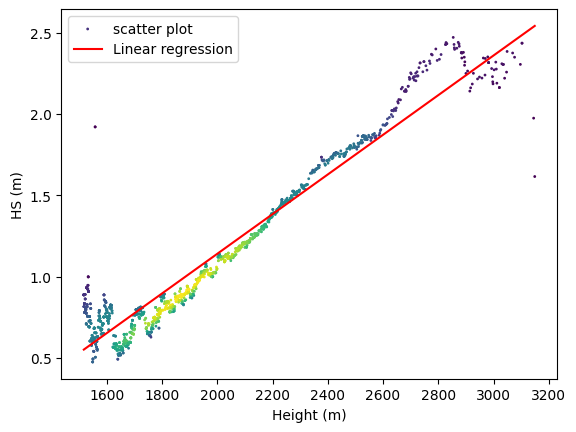
\includegraphics[width=\textwidth]{Slicing_after.png}
      \caption[Image 2]{}
      \label{fig:slicingb}
  \end{subfigure}
  \caption[Images]{Snow depth versus elevation in the Davos region (2013): (a) original distribution and (b) after applying the segmentation technique. The color gradient represents point density, visualized as a probability density function according to Scott's Rule \cite{scott2015multivariate}.}
  \label{fig:slicing}
\end{figure*}

Linear regressions fitted to the original and segmented datasets yield the following relationships for Figures \ref{fig:slicinga} and \ref{fig:slicingb}, respectively:

\begin{equation}
        HS = 146 \times 10^{-5} \cdot h - 1.830
\end{equation}

\begin{equation}
        HS = 124 \times 10^{-5} \cdot h - 1.353
\end{equation}

\noindent where $h$ represents elevation and $HS$ denotes snow depth. Segmentation mitigates bias from uneven sampling density, providing a more accurate representation of snow-elevation patterns.

% In the original dataset, the non-uniform distribution of sampling points can introduce bias in the regression analysis, particularly in regions with high data density. The segmented snow analysis serves as a normalization method to address this limitation, providing a more balanced representation of the snow-elevation relationship.} 

\subsubsection{Directional Analysis of Snow Depth Distribution}

Segmented snow depth analysis in the Davos region reveals a consistent pattern: minimum snow depths cluster within a narrow aspect range, while maximum depths vary more widely in direction (see Fig. \ref{fig:AspectHS}a). This asymmetry indicates that certain topographical orientations consistently receive less snow, likely influenced by prevailing winds and solar radiation.
% Analysis of segmented snow depth data in the Davos region reveals a consistent pattern: minimum snow depths cluster within a narrow range of aspects, while maximum depths show greater directional variability (see Fig. \ref{fig:AspectHS}a). This asymmetric distribution suggests that certain topographical orientations consistently receive less snow accumulation, likely due to prevailing wind patterns and solar radiation effects.

\begin{figure}[htbp]
  \centering
  \begin{subfigure}{0.49\textwidth}
    \centering
    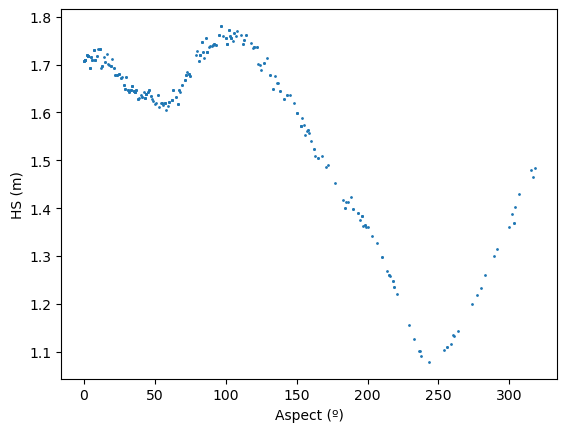
\includegraphics[width=\textwidth]{HSAspect.png}
      \caption{} \label{fig:HSAspect}
  \end{subfigure}
  %\hfill                              %% no blank line here.
  \begin{subfigure}{0.49\textwidth}
    \centering
    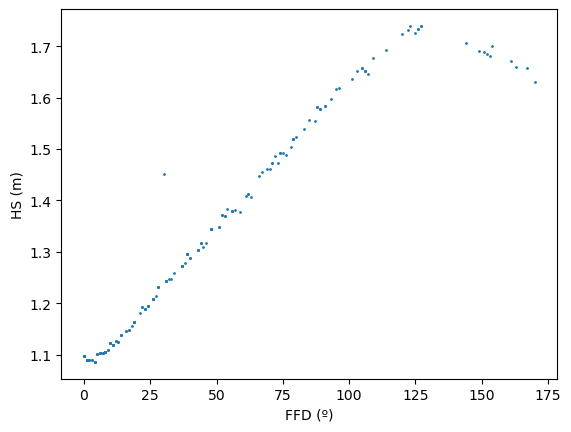
\includegraphics[width=\textwidth]{HSFFD(davos).png}
      \caption{} \label{fig:HSFFD}
  \end{subfigure}
  \caption{(a) Segmented snow depth (HS) versus surface aspect. (b) Segmented snow depth (HS) versus FFD.} \label{fig:AspectHS}
\end{figure}

To quantify this directional influence, we introduce the Far From $\Vec{D}$ (FFD) variable, where $\Vec{D}$ represents the direction of minimum snow accumulation. Unlike the standard aspect, which references north (0°), FFD measures a slope's angular deviation from $\Vec{D}$ to better align with the physical processes shaping snow distribution. %This approach aligns the coordinate system with the physical processes driving snow distribution establishing a meaningful reference direction.
Calculating FFD begins by determining $\Vec{D}$: an analysis of aspect and segmented snow depth across the study area identifies a consistent minimum snow depth direction between 150º and 360º. Using Taylor's theorem, we fit a polynomial to this region to precisely locate the minimum. This analysis yields $\Vec{D} = 245^{\circ} \pm 3^{\circ}$, representing the aspect associated with minimum snow accumulation.

For each slope in our study area, we then compute FFD as:

\begin{equation}
        \text{FFD} = |\alpha - \Vec{D}| \mod 180^{\circ}
\end{equation}

\noindent where $\alpha$ is the slope's aspect. The modulo operation constrains values to the range $[0^{\circ}, 180^{\circ}]$, with 0° aligning with $\Vec{D}$ (minimum snow) and 180° representing maximum deviation. While this transformation omits the directional sign (east or west relative to $\Vec{D}$), our analysis shows that the magnitude of deviation primarily governs snow accumulation (see Fig. \ref{fig:AspectHS}b). 

The stability of $\Vec{D}$ across the study area indicates that regional-scale processes, such as prevailing wind patterns, influence this directional dependency, validating FFD as a relevant predictor variable in snow depth models.

\subsection{Topographic position index} \label{sec_tpi}

The topographic position index (TPI) measures the elevation of the raster grid cell compared to the elevation of a specified number of neighboring cells obtained from DEMs. By definition, it determines concave and convex areas and therefore can predict whether an area is prone to snow accumulation. It has also been shown to be a good snow depth predictor \cite{revuelto2020random, daudt2023snow}. TPI can be calculated as the difference between a central point's elevation and its surrounding points' average elevation within a defined radius. The method of calculating this difference may vary, so we tested the two algorithms described below to determine which approach provides better snow depth prediction. Note that the first algorithm uses normalization, which may reduce the impact of extreme values but could mask important local variations. In contrast, the second algorithm utilizes direct elevation differences, potentially preserving local topographic features relevant to snow accumulation.

\begin{itemize}
    \item The first algorithm is available in the WhiteBoxTools library \cite{lindsay2014whitebox} and is based on the study by Newman et al. \cite{newman2018evaluating}. It is referred to as TPI throughout the rest of the manuscript. Notice that this algorithm returns normalized values in the range $[-1, 1]$ according to:
    \begin{equation}
        \text{TPI} =
        \begin{cases}
            \frac{z - \mu}{\mu - z_{\text{min}}} & \text{if } z < \mu \\ 
            \frac{z - \mu}{z_{\text{max}} - \mu} & \text{if } z \geq \mu
        \end{cases}
    \end{equation}
    \noindent where $z$ represents the elevation, $\mu$ stands for the average elevation, and $z_{\text{max}}$ and $z_{\text{min}}$ are the maximum and minimum elevations, respectively.
    
    \item The second method (TPI-Alt) calculates the absolute elevation differences using a moving window approach and can be expressed as:
    \begin{equation}
            \text{TPI-Alt} = z - \frac{\sum_{i,j \in W} w_{i,j}z_{i,j}}{\sum_{i,j \in W} w_{i,j}}
    \end{equation}
    \noindent where $z$ is the central cell elevation, $W$ represents the window of neighboring cells within the specified radius, $w_{i,j}$ are the spatial weights (1 in our implementation), and $z_{i,j}$ are the elevation values of the neighboring cells. We filter the results by limiting the maximum and minimum values to $\pm5$, treating values outside this range as outliers. This step ensures that extreme values are removed before further analysis.
\end{itemize}

\subsection{Snow cover extent}

Snow cover extent (SCE) is a probabilistic map designed to indicate the snow distribution across a given area. The SCE maps %, as depicted in Fig. \ref{fig:testDavos}
represent a fusion of diverse geospatial data sources weighted according to their robustness, accuracy, and resolution. Wegaw's methodology, following the approach by Grizonnet \cite{grizonnet2017operational}, involves computing the likelihood of snow cover for individual cells within a 20m x 20m grid. SCE is derived from optical satellite imagery utilizing the 'Let it Snow' (LIS) algorithm, as outlined by Gascoin et al. \cite{Gascoin2019}, applied to data from Copernicus Sentinel-2\footnote{\url{https://land.copernicus.eu/pan-european/biophysical-parameters/high-resolution-snow-and-ice-monitoring}}  as the primary layer for snow cover extraction, and with data from NASA MODIS/VIIRS\footnote{\url{https://modis-snow-ice.gsfc.nasa.gov/?c=MOD10_L2}} satellites serving as a secondary layer. 

To improve accuracy, cloud-covered grid cells are identified and removed from analysis through the atmospheric correction processor (Sen2Cor), following the approach proposed by Main-Knorn et al. \cite{Main-Knorn2017}. Additionally, periods of prolonged cloud cover are addressed through the integration of precipitation and temperature data from the Global Forecasting System\footnote{\url{https://www.ncei.noaa.gov/products/weather-climate-models/global-forecast}}. In instances where Sentinel-2 imagery is unavailable, or where grid cells exhibit significant uncertainty regarding snow cover, a probability factor is applied based on historical snow presence from past seasons or days. Wegaw provided us with 153 SCE maps spanning from 2017 to 2020.

\subsection{Dynamic snow depth measurements}
\label{subsec:temporalvars}

Dynamic variables can enhance the model's fit to predictions for specific dates due to their capacity to capture temporal variability. In this case, we utilize measurements of snow depth recorded at specific dates and locations by meteorological stations. Wegaw provided us with data within the area of interest spanning from 2017 to 2021 (Data from the Institute for Snow and Avalanche Research © 2023). Given the dispersed nature of the data\footnote{\url{https://s.geo.admin.ch/qj8e0lg568hj}}, we employ three different integration methods detailed below.

\begin{itemize}
    \item \textbf{DEMStat}: It is derived by the linear correlation between DEMs and snow depth at a macro scale \cite{Grunewald2014}. By applying linear regression to the DEM data, we introduce a new feature, $\text{DEMStat}$, which depends on station data and allows us to incorporate the desired temporal variability. The relationship is mathematically represented as:
    \begin{equation}
    \text{$SD_{i}$} = \alpha \cdot h_j + \beta
    \end{equation}
    \noindent where $h_j$ represents the elevation of the closest meteorological station, and \text{$SD_{i}$} denotes the snow depth at point $i$. %Using the fit method,
    Note that the linear regression model from the \textit{scikit-learn} library \cite{kramer2016scikit} was applied to estimate the coefficients $\alpha$ and $\beta$. This approach, however, may oversimplify local variations by relying solely on data from the closest station and potentially overlooking relevant information from other nearby stations.
    
    \item \textbf{Voronoi}: We spatially partition the data using Voronoi diagrams to identify the most applicable meteorological station. %The second method employs Voronoi diagrams for spatial partitioning. 
    Given a set of $n$ points $P = \{p_1, p_2, ..., p_n\}$ in the Euclidean plane, the Voronoi diagram of $P$ %, denoted by $Vor(P)$,
    is a partition of the plane into $n$ regions, where each region is associated with one point of $P$. Formally, for each point $p_j \in P$, its Voronoi region $V(p_j)$ is defined as:

    \begin{equation}
    V(p_j) = 
    \{ q \in \mathbb{R}^2: \|q - p_j\| \leq \|q - p_k\|, \forall p_k \in P, k \neq j \}
    \end{equation}

    Specifically, $V(p_j)$ comprises all points in the plane that are closer to $p_j$ than to any other point in $P$. In our context, each point $p_j$ in $P$ corresponds to the position of a measurement station, and the value of the snow depth collected by the sensor of that station is assigned to each point in the Voronoi region $V(p_j)$: 

    \begin{equation}
    \text{SD}_{V(p_j)} = \text{SD}_{p_j}
    \end{equation}

    This approach is particularly effective for preserving measured values at station locations and establishing clear boundaries of influence for each station. However, it can result in abrupt transitions at regional boundaries and may not fully capture the impact of topography on snow distribution. 
    
    \item \textbf{ProbStat}: This feature is designed to smooth discontinuities between adjacent meteorological stations and improve representation in areas distant from measurement points by incorporating influences from multiple stations. However, similar to the Voronoi method, it may not fully account for topographic effects on snow distribution. Mathematically, this feature is defined as follows:

    \begin{equation}
            \text{$SD_{i}$} = \frac{\sum_j^N SD_j/d_j}{\sum_j^N 1/d_j}
    \end{equation}
    \noindent where $SD_j$ represents the snow depth measurement at station $j$, $d_j$ denotes the distance from $i$ to the station $j$, and $N$ stands for the number of stations.
\end{itemize}

\section{Methods}
\label{Sec:Methodology}

This section presents MAPunet, a customized architecture based on the popular U-Net to generate snow depth maps through pixel-wise regression; and MAPchete, a library containing map generators used to obtain overlapped tiles from geospatial data.

\subsection{MAPunet architecture}

MAPunet is a pixel-wise regressor specifically designed to obtain snow depth maps from geospatial data sources. Formally, the primary objective of MAPunet is to learn a mapping function $f: V \rightarrow M$, defined as follows:

\begin{itemize}
    \item $V$ denotes a three-dimensional input volume with dimensions $(H, W, N)$, extracted from geospatial data, where $(H, W)$ represents the spatial dimensions and $N$ stands for the number of input features per spatial location.
    \item $M$ denotes a two-dimensional matrix of spatial dimensions $(H, W)$, in which each element $M_{i,j} \in \mathbb{R}^+$ represents the estimated snow depth at the spatial location $(i, j)$.
\end{itemize}

The architecture of our pixel-wise regressor, devised to learn the function $f$, is inspired by the popular U-Net \cite{ronneberger2015u}, known for its effectiveness in image segmentation tasks. Therefore, it consists of the following main components: (1) an encoder, composed of a sequence of convolutional and max-pooling layers aimed at gradually reducing the spatial resolution of the input while retaining essential features; (2) a decoder, composed of convolutional and up-sampling layers aimed at reconstructing the snow depth maps; and (3) a bottleneck, which connects both the encoder and the decoder and facilitates the preservation of contextual information in the final stage. In addition, it includes the so-called skip connections that link each encoder layer to each decoder stage, allowing the network to capture both low- and high-level information and finally amalgamate them into snow depth maps.
 
The size of the architecture depends on two main hyperparameters: (1) the depth, which represents the number of max-pooling layers; and (2) the width, which stands for the factor by which the number of representative feature channels increases after each convolutional block. In this research, the number of channels is defined as $2 \times \text{width} \times \text{depth}$.

Since the architecture is specifically designed to solve a regression problem, and in particular to predict snow depths, the output layer does not include any activation function to obtain continuous values. Regarding the loss function, it is important to note that, in geospatial maps constructed from various sources, we can find null input values for points lacking significant information. This scenario, referred to as sparse supervision \cite{lang2023}, occurs when only a subset of the target area has ground truth labels available for training. Although the supervision, in this case, may not be particularly sparse, the principle remains consistent: these null values should be ignored when calculating the loss function. For this reason, we define a masked loss function that handles missing data and can be used to train MAPunet:

\begin{equation}
    %\mathcal{L} = \sum_{i,j}^{N} (\hat{y}_{ij} - y_{ij})^2 \text{, } \forall y_{ij} \neq nodata
    \mathcal{L} = \sum_{i=1}^{H} \sum_{j=1}^{W} (\hat{y}_{ij} - y_{ij})^2 \text{, } \forall y_{ij} \neq nodata
    \label{Eq:masking}
\end{equation}

\noindent where $\hat{y}$ is the model's prediction, $y$ denotes the ground truth, $(H, W)$ represents the spatial dimensions of the input data, and $nodata$ stands for missing data.

\subsection{MAPchete generator}
\label{subsec:mapchete}

MAPchete\footnote{\url{https://github.com/abetatos/mapchete}} is a Python project designed to assist in the preparation of geospatial data for deep learning applications. It focuses on efficiently cropping large datasets into smaller tiles, aiming to create a dataset with minimum overlap between tiles --thereby preserving representativeness-- and preventing empty cells. LiDAR maps are known for their exceptional precision but often present challenges due to their empty cells, commonly referred to as \textit{nodata} values, that can be attributed to sensor limitations, occlusions, or data gaps. To counteract the high density of \textit{nodata} values, which could negatively impact model training, two algorithms were developed with the MAPchete library. With them, images are defined as tiles, or windows, composed of $N\times N$ grid cells, which serve as the input for our learning models:

\begin{itemize}
\item RANDchete involves randomly cropping rasters into tiles.
\item MAXchete is an optimization algorithm designed to ensure a homogeneous representation across a map. It employs an iterative process to track the selection frequency of each cell. In each iteration, the map is divided into overlapping sampling windows with dynamically adjusted spacing. The algorithm calculates the cumulative frequency of cells within each window and selects the one with the least sampling history, prioritizing underrepresented areas. Once a window is selected, frequency counts for all its cells are updated, maintaining a record of the spatial sampling distribution. This process continues until the desired average sampling density is achieved. To ensure data quality, the algorithm includes a threshold for acceptable missing data within each window, excluding those that exceed this threshold while still considering them in future selections. Overall, this approach normalizes the representation of all areas while adapting to the specific limitations of the input data.
\end{itemize}

\section{Experimental setup} \label{Sec:ExperimentalSetup}

The experiments were carried out on an AMD Ryzen 7 7700X 8-Core processor and a NVIDIA GeForce RTX 4070 with 12GB of VRAM. For the implementation, we used Python as the primary programming language, making use of PyTorch \cite{collobert2011torch7} and the following open-source libraries: RichDEM \cite{RichDEM}, to compute the slope and the aspect variables; Whiteboxtools \cite{lindsay2014whitebox}, to compute the TPI function; and Rasterio \cite{Rasterio}, GDAL \cite{GDAL}, and QGIS \cite{QGISsoftware} for data preprocessing and analysis. 

\subsection{Dataset}

The dataset used in this research covers a cumulative area of 1651 km$^2$ across three locations in Switzerland --Davos, Lauchernalp, and Saflischpass-- collected between 2010 and 2020. As detailed in Table \ref{table:areaoverview}, some maps cover the same areas but on different dates, with each survey capturing slightly varied extents. Consequently, while the total surveyed area is 1651 km², the largest single training area is 161.08 km², and the test area is 369.19 km².

\begin{table}[htbp]
\caption{Overview of the experimental area with multiple locations (2010-2022). The areas are calculated as the sum of the area of each cell, excluding those with $nodata$ values.}
\label{table:areaoverview}
\centering
\small
\begin{tabular}{lllr}
\hline
Partition & Location & Acquisition date  & Area (km$^2$)  \\ 
\hline
Train & Davos & 2010-04-16 & 122.51  \\ 
      & Davos & 2012-03-20 & 126.48  \\ 
      & Davos & 2013-04-15 & 125.71  \\ 
      & Davos & 2014-04-17 & 108.55  \\ 
      & Davos & 2015-04-20 & 109.31  \\ 
      & Davos & 2016-01-26 & 109.54  \\ 
      & Davos & 2016-03-09 & 109.96  \\ 
      & Davos & 2016-04-20 & 110.80  \\ 
      & Davos & 2020-04-06 & 34.47   \\ 
      & Davos & 2021-04-16 & 161.08  \\ 
\hline
Validation & Lauchernalp  & 2022-02-24 & 1.14  \\ 
    & Lauchernalp  & 2022-05-11 & 2.26  \\
    & Saflischpass  & 2022-05-12 & 4.48  \\ 
    & Saflischpass  & 2022-05-12 & 6.55  \\ 
\hline
Test & Davos  & 2017-03-16 & 369.19   \\ \hline
\end{tabular}
\end{table}

Figure \ref{fig:LidarCover} shows the three regions where the LiDAR surveys were conducted, highlighting the maximum spatial extent of the resulting snow depth maps. The data used are derived from two LiDAR data sources, described below.

\begin{itemize}
    \item Eight snow depth maps were collected from 2010 to 2016 in the Swiss region of Davos. These data are publicly available on Envidat\footnote{\url{https://www.envidat.ch/dataset/snow-depth-mapping}} \cite{Bhler2015}. Snow depth mapping was performed using the ADS80 optoelectronic scanner, acquiring stereo imagery with a spatial resolution of 0.25 m to generate digital surface models (DSM) of winter and summer terrains. The snow depth maps have a 2 m resolution with a vertical depth accuracy of $\pm$30 cm (RMSE) in complex alpine topography. The overall accuracy of the snow depth maps is better than 15\% when compared to the average snow depth of 2.2 m over the entire test site, as validated against independent data such as manually measured snow plots, dGNSS points, terrestrial laser scanning, and ground-penetrating radar data. Figure \ref{fig:satelliteDavos} provides a visual representation of the data coverage from 2014 for further context.
    
    \item Nine snow depth maps were collected from 2017 to 2020 in the Swiss regions of Davos, Lauchernalp, and Saflischpass. The data used for this study was collected by the Institute for Snow and Avalanche Research \cite{Buhler2023, Buhrle2023} and sold privately to Wegaw. The high-resolution snow depth maps were produced using aerial photogrammetry with the Vexcel UltraCam Eagle Mark 3 camera and compared to snow-off digital terrain models obtained from Airborne Laser Scanning (ALS). The accuracy of these snow depth maps was validated using multiple methods: independent checkpoints to ensure the correct orientation of the digital surface models (DSMs), comparison with DSMs from unpiloted aerial systems (UAS), providing high-accuracy references over small areas, and comparison of snow-free pixels with ALS data to assess possible misalignments. The results show a RMSE of 0.25 m for the UltraCam X and 0.15 m for the UltraCam Eagle M3, highlighting improvements in accuracy over time. Figure \ref{fig:LidarCover} provides a comprehensive overview of the study area in the Davos region.
\end{itemize} 

\begin{figure}[htbp]
    \centering
    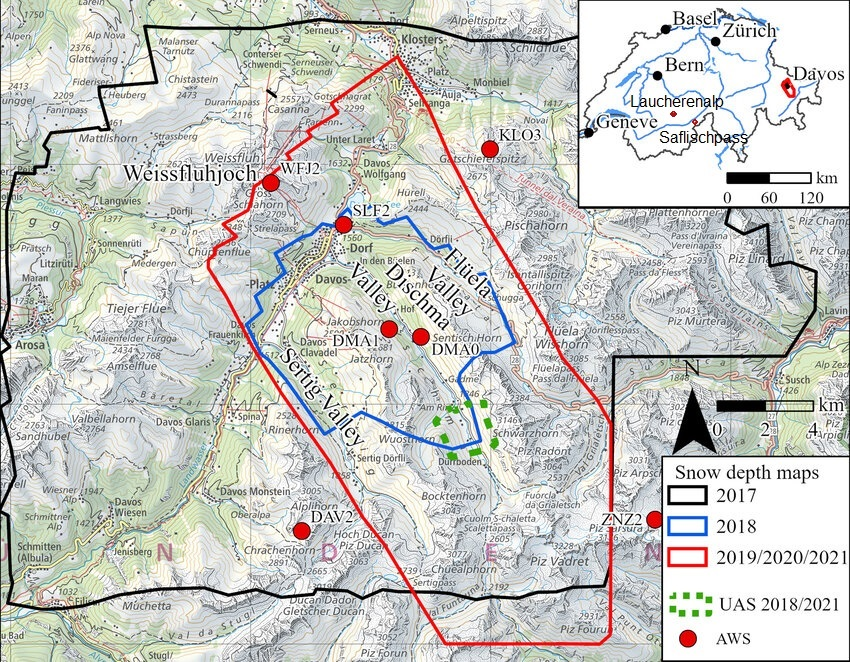
\includegraphics[width=1\columnwidth]{StudyArea2.png}
    \caption{Study area overview: The 2017 snow depth map (test area) generated from the airplane imagery is shown in black, with the 2018 map in blue and the 2019–2021 maps (training area) in red. Green areas represent UAS reference data from 2018 and 2021. Red points mark Automatic Weather Stations (AWS) for precise snow depth measurements. The inset map shows the 2019–2021 flight areas in Switzerland, with red dots indicating the regions of Lauchernalp and Saflischpass. Map source: \cite{Buhrle2023}.}
    \label{fig:LidarCover}
\end{figure}

The RANDchete method was initially applied to extract the tiles from these maps. However, to improve dataset quality and ensure comprehensive geographic representation, we finally used MAXchete. The frequency of each grid cell's appearance in the dataset was set to 4, effectively serving as a data augmentation strategy that increases the representation and variety of training images. Fig. \ref{fig:mapchetedensity} illustrates the differences between the two algorithms available in the MAPchete library.

\begin{figure}[htbp]
    \centering
    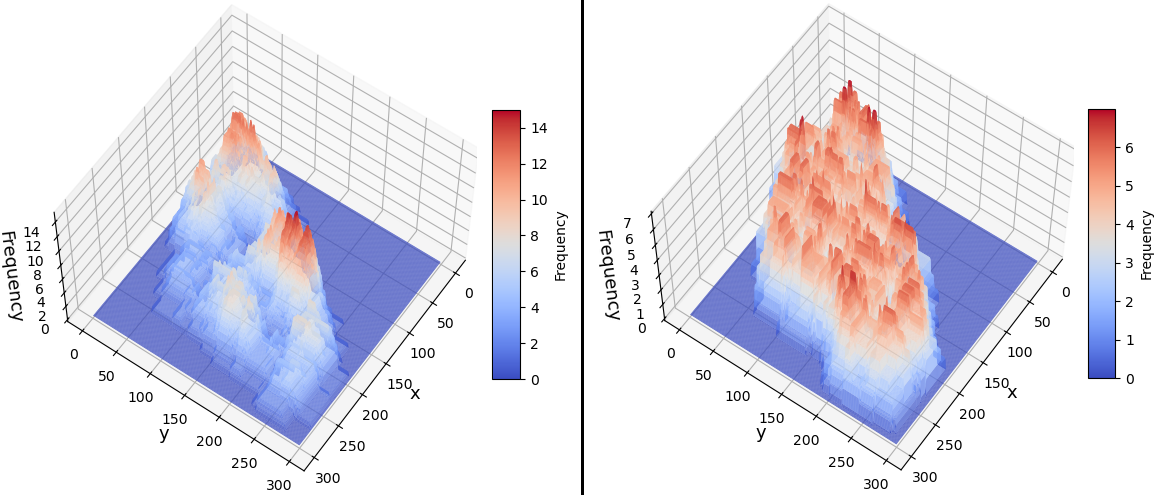
\includegraphics[width=1\columnwidth]{MAPchete.png}
    \caption{%The number of times a given cell appears in the final dataset after 100 iterations in the Saflischpass zone is shown, with the random approach (RANDchete) represented on the left and the optimization algorithm (MAXchete) on the right. 
    Frequency of cell appearances in the final dataset after 100 iterations in the Saflischpass zone: the random approach (RANDchete) is shown on the left and the optimization algorithm (MAXchete) on the right. The x and y axes denote the local spatial coordinates of cells in a grid covering the Saflischpass area, where each point represents a specific cell where the algorithm was applied.}
    \label{fig:mapchetedensity}
\end{figure}

For a given frequency (4 in our specific application), the number of tiles depends on their size. As can be seen in Table \ref{table:Ntiles}, different configurations led to different
numbers of images in our dataset. In this research, the tiles were set at a resolution of $256 \times 256$, chosen for their balance between spatial coverage and manageable dataset size. The EPSG:2056 coordinate system was employed given that it covers Switzerland using meters as units. Moreover, each input feature was resized to a uniform resolution of 5m, driven by the availability of high-resolution 2m LiDAR maps. Resampling was carried out using GDAL's Warp function with bilinear interpolation, specifying both horizontal and vertical resolutions (xRes=5, yRes=-5).

\begin{table}[htbp]
\centering
\caption{Number of tiles depending on their dimensions.} \label{table:Ntiles}
\begin{tabular}{ll}
\hline
Size & No. of tiles \\ \hline
$512 \times 256$ & 1353 \\
$256 \times 256$ & 5333 \\
$128 \times 128$ & 21145 \\
\hline
\end{tabular}
\end{table}

In geospatial analysis, data is often divided into sequential tiles, which can create discontinuities along tile boundaries when reconstructing a complete map. However, the MAPchete algorithm generates overlapping tiles, allowing us to mitigate this by spatially averaging predictions across tiles. %However, due to the nature of the MAPchete algorithm, we obtain tiles that do overlap, and thus we can avoid the behavior mentioned above by averaging the predicted tiles over space. 
After extracting tiles from the ground-truth maps, we computed the ten features described in Section \ref{Sec:Features}, assigning each grid cell a value that encapsulates the distinctive features of its geographic area. 

% Finally, for experimental purposes, the dataset was split into training (66.4\%), validation (4.8\%), and test (28.4\%) sets. A more detailed description, including the different locations and the dates} of data acquisition, is provided in Table \ref{table:areaoverview}. 
For experimental purposes, the dataset was divided into training (66.4\%), validation (4.8\%), and test (28.4\%) sets. See Table \ref{table:areaoverview} for details on the split, along with additional information on locations and data acquisition dates.  To ensure geographic diversity and prevent overfitting, the validation partition includes regions outside the study area, specifically Lauchernalp and Saflischpass, which were used for model hyperparameter fitting and other validation tasks. Both the training and test data were sourced from the target study area (Davos), but from different years, allowing us to evaluate the model's ability to predict snow depth at unseen times. Notably, the test area is substantially larger than the training area, being two to three times its size in some cases (as shown in Figure \ref{fig:lidarDavos} and Table \ref{table:areaoverview}), which allows for evaluating the model's ability to generalize across different geographic areas.

\begin{figure}[htbp]
  \centering
  \begin{subfigure}{0.48\textwidth}
    \centering
    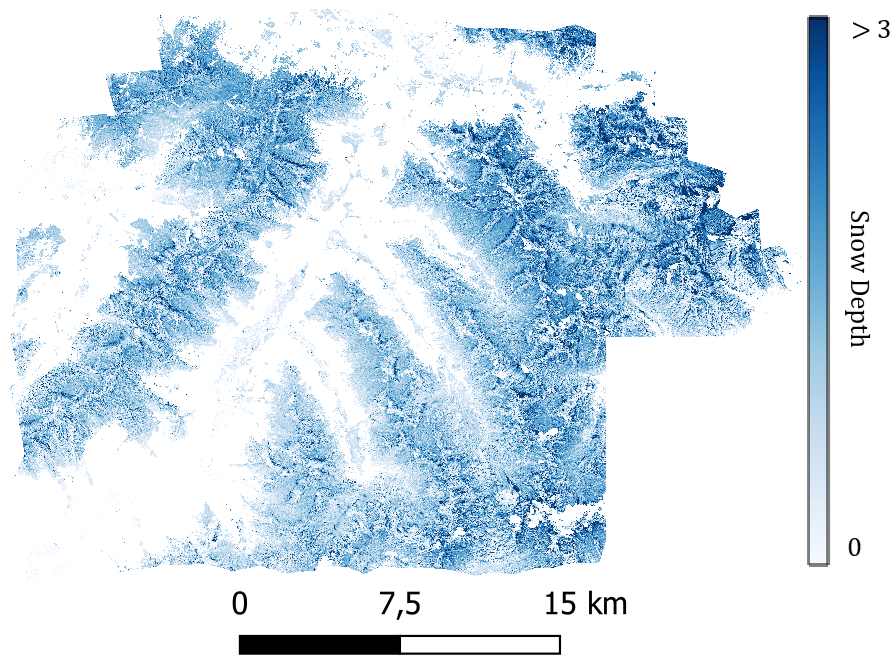
\includegraphics[width=\textwidth]{DAVOS_mod.png}
      \caption{} \label{fig:testDavos}
  \end{subfigure}
  %\hfill                              %% no blank line here.
  \begin{subfigure}{0.48\textwidth}
    \centering
    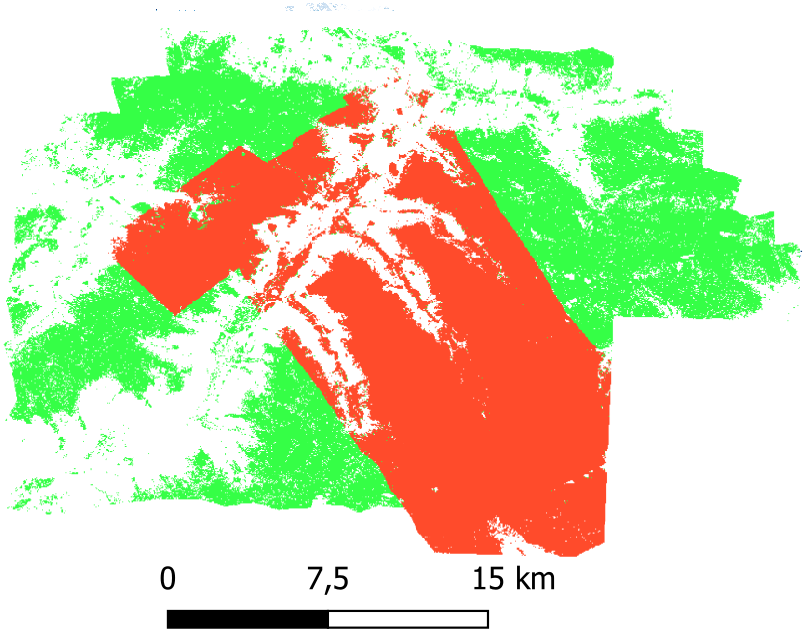
\includegraphics[width=\textwidth]{DavosLIDAR-2017-Rest.png}
      \caption{} \label{fig:lidarDavos}
  \end{subfigure}
   \hfill                              %% no blank line here.
   \begin{subfigure}{1\textwidth}
    \centering
    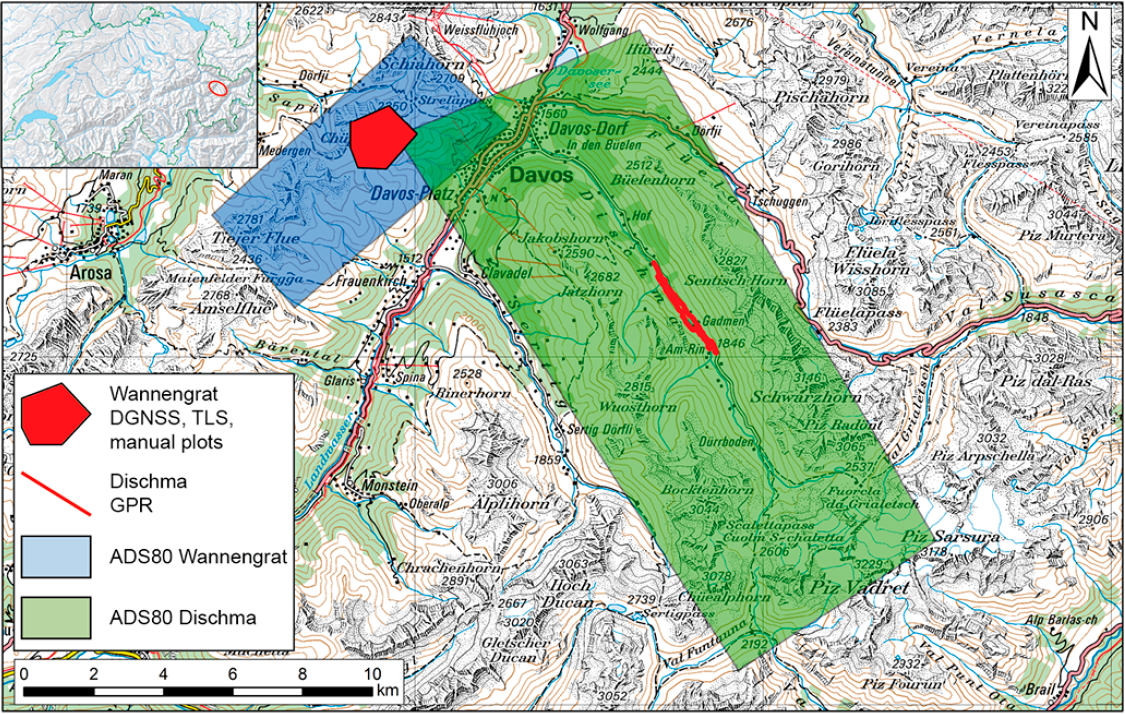
\includegraphics[width=\textwidth]{Davos2014Area.PNG} % Replace with your satellite image filename
      \caption{} \label{fig:satelliteDavos}
  \end{subfigure}
  \caption{(a) Representative example from our dataset for the Davos area (2017), including the test region and a snow depth scale with a maximum value of 3 meters. (b) Map showing the areas covered by LiDAR flights in the Davos region, including the training areas (in red) and the test areas (in green and red). (c) ADS80 data coverage and locations of the reference datasets at Wannengrat and the Dischma Valley, Davos, Switzerland (2014). Map source: \cite{Bhler2015}.} \label{fig:davosDataset}
\end{figure}

\subsection{Hyperparameter configuration} \label{subsec:hyperparams}

Table \ref{tab:hyperparameters} summarizes the hyperparameter settings obtained after a grid search optimization process, where various combinations of hyperparameters were systematically tested. The model's performance was evaluated by comparing the predicted maps to the ground truth using the average error, ensuring the reproducibility of the results.

\begin{table}[htbp]
\centering
\caption{Hyperparamter values selected for the best-performing model.} \label{tab:hyperparameters}
\begin{tabular}{ll}
\hline
Hyperparameter & Value \\ \hline
Input size & $256 \times 256$ \\
Batch size & 128 \\
MAPunet depth & 7\\
MAPunet width & 12 \\
Optimizer & SGD + Adam \\
Learning rate & $10^{-3}$\\ 
Momentum & 0.9 \\
Weight decay & $10^{-5}$ \\
Number of epochs & 15 \\
\hline
\end{tabular}
\end{table}

% We conducted a study aiming to identify the best hyperparameters for our architecture, utilizing TPI, SCE, DEM, aspect, and slope as input variables. 
We observed that increasing the depth of the model results in improved performance. The max-pooling layer, which reduces the spatial resolution (width $\times$ height) by half at each step, was configured with the maximum depth value (7) for an input image of $256 \times 256$.

Subsequently, we explored the impact of varying the channel width among the values 5, 7, 10, 12, 15, and 20. The average error indicated that a larger width does not necessarily produce better results, with 12 being the selected option. This configuration showed an error reduction of 6\% compared to the second-best alternative for the width (10).

As part of the training stage optimization process, we employed a two-stage approach, combining stochastic gradient descent (SGD) \cite{kiefer1952stochastic} and Adam \cite{kingma2014adam}. Initially, SGD was used for the first 15 epochs to locate a stable local minimum. After this, we switched to Adam to further refine the optimization within that region. This approach was chosen based on our observations that using Adam from the start could lead to instability, while introducing Adam after the SGD phase resulted in improved performance. Note that for SGD, we used a momentum of $0.9$, a weight decay of $10^{-5}$, and a learning rate of $10^{-3}$; while for Adam, we used a learning rate of $10^{-3}$.

\subsection{Performance metrics} \label{Sec:Metrics}

To evaluate the performance of the proposed MAPunet architecture, we have considered three commonly used metrics for pixel-wise regression.

\begin{itemize}
    \item The mean absolute error (MAE) measures the average magnitude of errors between predicted and actual values. MAE is defined as:
    \begin{equation}
    \text{MAE} = \frac{1}{n} \sum_{i=1}^{n} |y_i - \hat{y}_i|
    \end{equation}
    \noindent where $n$ is the number of data points, $y$ is the actual snow depth, and $\hat{y}$ is the predicted snow depth.

    \item The root mean square error (RMSE) measures the square root of the average of the squared differences between predicted and actual values. It is commonly used to detect predictions sensitive to extreme errors or outliers. RMSE is defined as:
    \begin{equation}
    \text{RMSE} = \sqrt{\frac{1}{n} \sum_{i=1}^{n} (y_i - \hat{y}_i)^2}
    \end{equation}
     \noindent where $n$ is the number of data points, $y$ is the actual snow depth, and $\hat{y}$ is the predicted snow depth.
    \item The $R^2$ score, also known as the coefficient of determination, measures how well the regression predictions approximate the real data points. $R^2$ is defined as:
    \begin{equation}
        R^2 = 1 - \frac{\sum_{i=1}^n (y_i - \hat{y}_i)^2}{\sum_{i=1}^n (y_i - \overline{y})^2}
    \end{equation}
    \noindent where $n$ is the number of data points, $y$ is the actual snow depth, $\hat{y}$ is the predicted snow depth, and $\overline{y}$ is the mean of the $y$ values. 
\end{itemize}

For clarity, when we mention errors in this manuscript, we refer to the MAE. The RSME is only reported in our final model for study comparability.

\section{Results} \label{Sec:Results}

This section analyzes variable informativeness and conducts an ablation study to identify a subset of variables that enable effective system testing on the available hardware. Finally, we analyze the dynamic variables and the error distribution.

\subsection{Topographic position index}

We comprehensively analyzed large-scale correlations to establish the ideal topographic position index (TPI). Since lower TPI values suggest areas where snow accumulates, an effective TPI may demonstrate a monotonically decreasing relationship with snow depth.

Figure \ref{fig:IPTHS} illustrates the observed trend in the behavior of the TPI, aligning with our defined criteria. To better represent the described data, we opted to fit the TPI to a sigmoid function due to its ability to capture this behavior accurately:

\begin{equation}
Y = \frac{a}{{1 + e^{c \cdot (X - d)}}} + b
\end{equation}

\noindent where \( Y \) represents the snow depth, \( X \) is the TPI, and \( a \), \( b \), \( c \), and \( d \) are parameters. The implementation was done via the \textit{optimize} module of the \textit{scikit-learn} library using the Trust Region Reflective algorithm \cite{Branch99}.

 \begin{figure}[htbp]
    \centering
    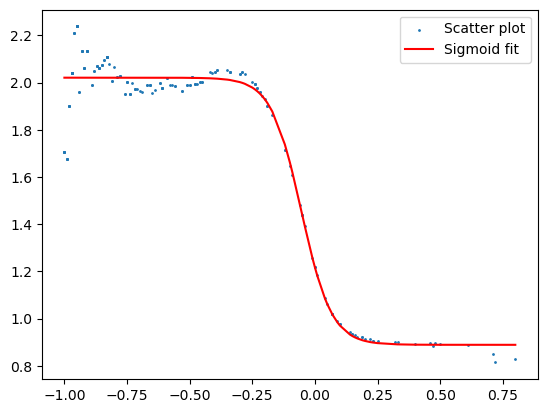
\includegraphics[width=0.8\columnwidth]{TPIdavos.png}
    \caption{Segmented snow depth (HS) vs. topographic position index (TPI).}
    \label{fig:IPTHS}
\end{figure}

As explained in Section \ref{sec_tpi}, the average elevation used in TPI is calculated based on a radius $r$ that defines the surrounding points involved. For this purpose, filters with dimensions $(2r+1) \times (2r+1)$ were considered. Among the filter sizes analyzed, $\{5, 7, 9, 11, 13, 22, 50\}$, we opted for the one with the highest coefficient of determination, $R^2$. Our analysis revealed that 11 was the optimal value for both TPI functions.

\subsection{Informativeness of the input variables} \label{subsec:informativity}

The next experiment aims to determine which of the input variables is the most informative. Table \ref{Table:LOO} shows the results of an ablation study, in which we trained a model and evaluated it on the validation set by systematically omitting one variable at a time. In some cases, two variables were excluded due to their correlation: DEM and DEMStat, and TPI and TPI-Alt. 

\begin{table}[htbp]
\caption{MAE (in meters) in validation obtained from the ablation study, with all variables included except the one indicated. The best result is in bold.}
%Average errors (in meters) achieved in the ablation study, using all variables except the one shown.
\label{Table:LOO}
\centering
\resizebox{\linewidth}{!}{%
\begin{tabular}{cccccccccc}
\hline
DEMStat & \begin{tabular}[c]{@{}c@{}}DEM \&\\ DEMStat\end{tabular}  & FFD & Slope & TPI-Alt & DEM & Aspect & SCE & \begin{tabular}[c]{@{}c@{}}TPI \&\\ TPI-Alt\end{tabular}& TPI \\ \hline
\textbf{0.528} & 0.529 & 0.536 & 0.539 & 0.546 & 0.548 & 0.558 & 0.560 & 0.561 & 0.570\\ \hline
%FFD & DEMStat & TPI-Alt & TPI & \begin{tabular}[c]{@{}c@{}}TPI \&\\ TPI-Alt\end{tabular} & Slope & Aspect & SCE & DEM & \begin{tabular}[c]{@{}c@{}}DEM \&\\ DEMStat\end{tabular} \\ \hline
%0.536 & \textbf{0.528} & 0.546 & 0.570 & 0.561 & 0.539 & 0.558 & 0.560 & 0.548 & 0.529 \\ \hline
\end{tabular}%
}
\end{table}

While the ablation results may initially suggest that DEMStat is not essential, this finding requires closer examination. The observed performance of the model without DEMStat does not imply that temporal information is unimportant; rather, it reflects limitations in our linear regression approach for incorporating station data, particularly given the sparse and uneven distribution of weather stations relative to the study area's large size (see Figure \ref{fig:LidarCover}). By contrast, studies in much smaller areas (e.g., $\sim$300 m x 1000 m) have relied on up to 16 stations to obtain robust results \cite{Geissler2023}.

Additionally, the specific locations of our stations --situated at elevations between 2000 and 3000 meters on flat, wind-sheltered terrain in avalanche-prone zones-- make it challenging to collect data that is broadly representative of the entire region. Relying solely on data from the nearest station through linear regression can therefore miss critical snow depth variations across such an extensive and topographically complex area. This limitation of DEMStat motivated our development of more sophisticated methods to capture temporal variability, namely the Voronoi and ProbStat approaches. These methods address spatial representation challenges and aim to improve snow depth mapping accuracy using available meteorological data.
% Moreover, it is important to consider the specific geographical settings of these stations: they are located between 2000 and 3000 meters altitude, on flat terrain protected from wind, and in avalanche-prone areas, as their primary purpose is to predict avalanches \footnote{\url{https://www.slf.ch/en/avalanche-bulletin-and-snow-situation/measured-values/description-of-automated-stations/}}. This implies that obtaining general and informative data from these stations --data that are representative of the entire region-- is challenging.
%Consequently, using data from the nearest single station through linear regression may not effectively capture snow depth variations across such a large region, especially given the complex topography and the significant distances between stations. The apparent limited utility of DEMStat in the ablation study actually motivated us to develop more sophisticated methods for incorporating temporal variability, namely the Voronoi and ProbStat approaches, which are further analyzed in Section \ref{subsec:otras_temp}. These methods aim to address the aforementioned issues and enhance the accuracy of the mapping process using meteorological station data.

Finally, it is worth mentioning that TPI is the variable that yields the best results. When TPI is excluded from the model, predictions worsen by 1 cm compared to the second most influential variable, SCE, with a corresponding error increase from 0.528 to 0.570 m when DEMStat is also removed. While this rise in error may appear minor, it represents an approximate 8\% increase, which is meaningful in the context of operational accuracy requirements for snow depth mapping. In conclusion, the variables identified as most influential are TPI, SCE, Aspect, DEM, Slope, and FFD.

% In summary, the best predictors are TPI, SCE, Aspect, DEM, Slope, and FFD.

\subsection{Input variable selection}

Taking into consideration the computational limitations, we undertake a selection process to identify the variables to be included in our final dataset. We prioritize variables based on their relevance to the research objectives and their potential impact on the study outcomes. To do this, we train the model through an iterative process by adding the variables one by one in the order determined by the previous experiment.

Table \ref{Tab:Iterative} displays the MAE on validation, showing a significant improvement that stabilizes around 0.53 m. With only TPI, SCE, aspect, and DEM, the error averages 0.532 m, representing a mere 0.002 m difference from the best model. Given this similarity, these variables seem sufficient to serve as a base for our subsequent experiments with dynamic measurements while maintaining computational efficiency. Henceforth, we refer to this configuration as the \textit{Efficient Set}.

\begin{table}[htbp]
\caption{ MAE (in meters) in validation obtained using the iterative strategy, where the most recently added variable is the one indicated. The best result is in bold.} 
\label{Tab:Iterative}
\centering
\begin{tabular}{lcccccccc}
\hline
TPI & SCE & Aspect & DEM & Slope & FFD & DEMStat \\ \hline
0.607 & 0.576 & 0.548 & 0.532 & 0.531 & 0.530 & \textbf{0.529} \\ \hline
\end{tabular}
\end{table}

\subsection{Dynamic snow depth measurements}
\label{subsec:otras_temp}

As detailed in Section \ref{subsec:temporalvars}, we introduce temporal variability into our model by proposing three new features. While linear regression (DEMStat) was used in previous sections, here we test the last two features: Voronoi and ProbStat. We then train two models with the Efficient Set. Incorporating Voronoi yields a validation MAE of 0.527 m, {while ProbStat slightly improves the error to 0.525 m. This results in a 0.93\% and 1.3\% reduction in error, respectively, compared to the model trained solely with the Efficient Set.

Based on these results, we select the model trained with the Efficient Set and ProbStat as our best model, achieving an MAE of 0.525 m and an RMSE of 0.634 m on validation. Finally, when evaluating this model on the test set, we observe a slight degradation in performance, with a final MAE of 0.62 m and an RMSE of 0.80 m.

%To analyze in detail the impact of ProbStat on our test set, we scale this feature with a mask of values of 0, 0.5, and 1, and then evaluate how the predictions deviate from the labeled dataset. Figure \ref{Fig:ProbStat} illustrates the behavior of ProbStat. As expected, more accurate ProbStat values tend to result in better predictions of snow depth.

\subsection{Error analysis}
\label{subsubsec:errordistr}

The analysis of the error distribution on the test set reveals significant patterns in the accuracy of the snow depth measurement system across various variables, as depicted in Figure \ref{fig:AbsErrorsVars}.

\begin{figure*}
  \centering
  % Primera fila
  \begin{subfigure}{0.49\textwidth}
    \centering
    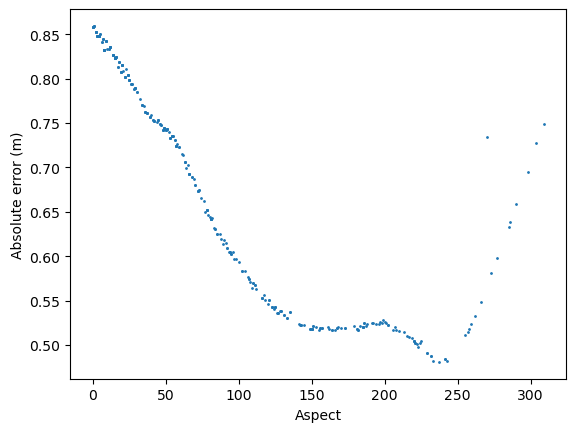
\includegraphics[width=\textwidth]{thumbnail_image (2).png}
    \caption[Image 1]{}
    \label{fig:AbsError2}
  \end{subfigure}
  \hfill
  \begin{subfigure}{0.49\textwidth}
    \centering
    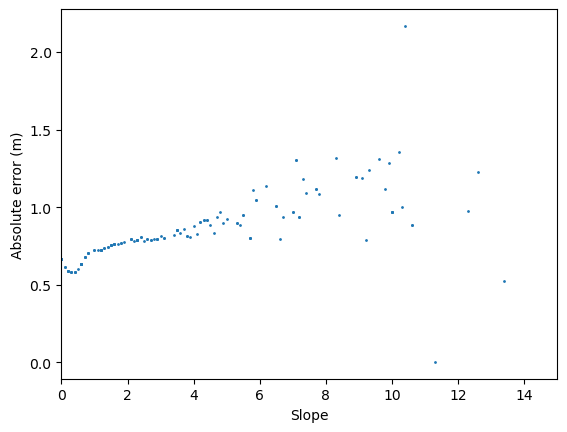
\includegraphics[width=\textwidth]{thumbnail_image (3).png}
    \caption[Image 2]{}
    \label{fig:AbsError3}
  \end{subfigure}
  
  \vspace{0.5cm} % Espacio vertical entre las filas
  
  % Segunda fila
  \begin{subfigure}{0.49\textwidth}
    \centering
    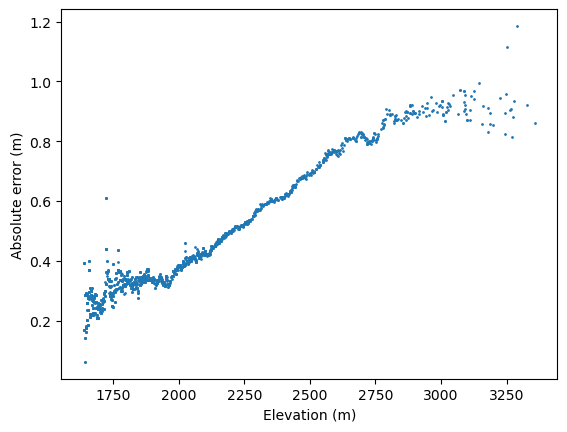
\includegraphics[width=\textwidth]{thumbnail_image (4).png}
    \caption[Image 3]{}
    \label{fig:AbsError4}
  \end{subfigure}
  \hfill
  \begin{subfigure}{0.49\textwidth}
    \centering
    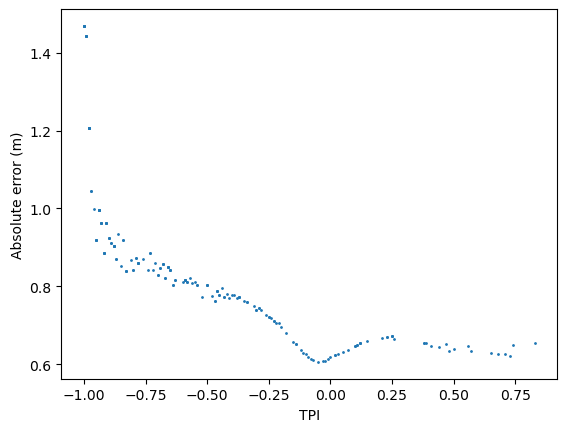
\includegraphics[width=\textwidth]{thumbnail_image (5).png}
    \caption[Image 4]{}
    \label{fig:AbsError5}
  \end{subfigure}
  
  \vspace{0.5cm} % Espacio vertical entre las filas
  
  % Tercera fila
  \begin{subfigure}{0.49\textwidth}
    \centering
    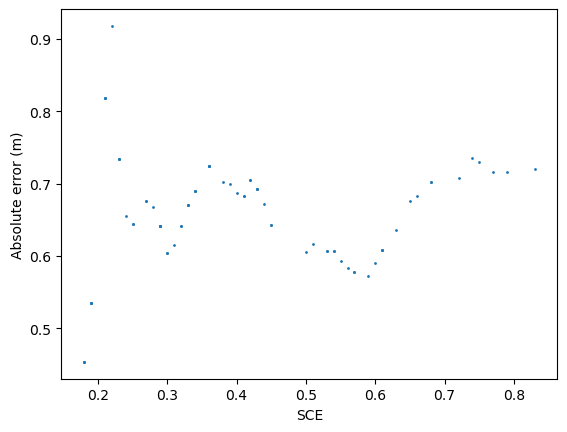
\includegraphics[width=\textwidth]{thumbnail_image (6).png}
    \caption[Image 5]{}
    \label{fig:AbsError6}
  \end{subfigure}
  \hfill
  \begin{subfigure}{0.49\textwidth}
    \centering
    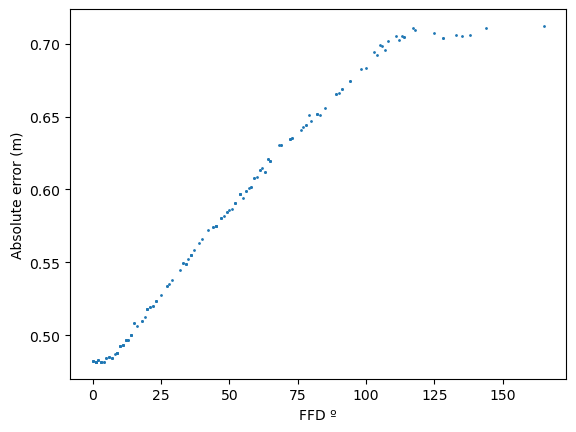
\includegraphics[width=\textwidth]{thumbnail_image (7).png}
    \caption[Image 6]{}
    \label{fig:AbsError7}
  \end{subfigure}
  \caption[Images]{Error distribution relative to: (a) Aspect, (b) Slope, (c) Elevation, (d) Topographic Position Index (TPI), (e) Snow Cover Extent (SCE), and (f) Far From $\Vec{D}$ (FFD) in the test set.}
  \label{fig:AbsErrorsVars}
\end{figure*}

\begin{itemize}
    \item Aspect (Figure \ref{fig:AbsError2}) shows a clear trend, with maximum error (approximately 0.85 m) occurring at low values (near 0°), gradually decreasing to a minimum of around 0.5 m between 150° and 250°, indicating greater precision on south and southwest-facing slopes. % Regarding aspect, (Figure \ref{fig:AbsError2}), a clear trend is observed where the error is maximum (approximately 0.85 m) at low values (near 0°), gradually decreasing to reach a minimum (around 0.5 m) between 150° and 250°. This finding suggests that the system offers greater precision on south and southwest-facing slopes.
    
    \item Slope (Figure \ref{fig:AbsError3}) notably influences measurement accuracy, with minimal error (about 0.6 m) on nearly flat surfaces, which increases rapidly up to 2° slopes and more gradually up to 6°. For slopes greater than 6°, high variability in error is observed, with some measurements reaching up to 2.2 m, suggesting the system is more reliable on flat or gently sloping terrain. % Terrain slope shows a notable influence on measurement accuracy  (Figure \ref{fig:AbsError3}). The error is minimal (about 0.6 m) on nearly flat surfaces, increasing rapidly up to 2° slopes and then more gradually up to 6°. For slopes greater than 6°, high variability in error is observed, with some points reaching up to 2.2 m. These results indicate that the system is more reliable on flat or gently sloping terrain, while steep slopes present significant challenges for measurement accuracy.
     
     \item Elevation (Figure \ref{fig:AbsError4}) has a clear positive correlation with absolute error, where accuracy is highest (approximately 0.2 m) at the lowest elevations (around 1700 m), increasing steadily to 0.8--1.0 m at higher elevations (near 3250 m), indicating performance deterioration at greater heights. % Elevation demonstrates a clear positive correlation with absolute error (Figure \ref{fig:AbsError4}). Measurements are most accurate (error of approximately 0.2 m) at the lowest elevations (around 1700 m), and the error increases steadily with height, reaching values of 0.8-1.0 m at the highest elevations (near 3250 m). This trend suggests that system performance deteriorates at higher altitudes, possibly due to more challenging conditions.}
     
     \item Topographic Position Index (TPI) (Figure \ref{fig:AbsError5}) analysis reveals that error is highest (up to 1.5 m) at strongly negative TPI values (around -1.0) but decreases rapidly as TPI increases to about -0.25, with the best performance occurring for values between -0.25 and 0.75, suggesting measurements are more accurate on relatively flat or slightly elevated terrain. % The Topographic Position Index (TPI) reveals that the error is highest (up to 1.5 m) at strongly negative TPI values (around -1.0) (Figure \ref{fig:AbsError5}), decreasing rapidly as TPI increases to about -0.25. The system shows its best performance and greatest consistency for TPI values between -0.25 and 0.75. These findings indicate that measurements are more accurate on relatively flat or slightly elevated terrain, and less reliable in depressions or valleys.
     
     \item Snow Cover Extent (SCE) (Figure \ref{fig:AbsError6}) does not show a clear trend in relation to measurement error. While a slight decrease is observed for SCE values between 0.5 and 0.6, the large variability across this range suggests that other factors may have a more significant impact on accuracy. % Regarding Snow Cover Extent (SCE), (Figure \ref{fig:AbsError6}), no strong and clear trend is observed in relation to measurement error. Although a slight decrease in error is noted for SCE values between 0.5 and 0.6, the high variability present across the entire range of SCE suggests that other factors may have a more significant influence on measurement accuracy.
     
     \item Far From $\Vec{D}$ (FFD) (Figure \ref{fig:AbsError7}) analysis shows a strong positive correlation with absolute error, displaying a nearly linear increase as FFD rises from 0° to approximately 125°, with minimal error (around 0.48 m) occurring when FFD is close to 0°. As FFD increases, errors peak at about 0.72 m around 150°, suggesting the system performs best when slopes align with the direction of minimum snow accumulation. % The analysis of the FFD variable reveals a strong positive correlation with the absolute error in snow depth measurements. FFD, calculated by rotating the aspect towards the minimum snow direction, provides insight into how the orientation of the terrain relative to the direction of minimum snow accumulation affects measurement accuracy. The graph shows a clear and nearly linear increase in absolute error as FFD increases from $0^{\circ}$ to approximately $125^{\circ}$. The error is minimal (around 0.48 m) when FFD is close to $0^{\circ}$, indicating that measurements are most accurate when the aspect aligns closely with the direction of minimum snow accumulation, $\vec{D} = 245^{\circ} \pm 3^{\circ}$. As FFD increases, the error steadily rises, reaching a maximum of about 0.72 m at FFD values around $150^{\circ}$.
\end{itemize}

%This trend suggests that the snow depth measurement system performs best on slopes that face the direction of minimum snow accumulation, likely due to more consistent and predictable snow distribution patterns in these areas. Conversely, as the aspect deviates further from this optimal direction, measurement errors increase, likely due to more complex snow accumulation and redistribution processes on these slopes.}

%The strong correlation between FFD and absolute error underscores the importance of considering terrain orientation in snow depth measurements. It also validates the utility of the FFD variable in capturing additional information about the relationship between aspect and measurement accuracy, particularly for lower snow depths where the impact of aspect appears to be more pronounced.}

In conclusion, this analysis demonstrates that the snow depth measurement system performs optimally on gentle to moderate slopes, at lower elevations, with aspects ranging from 150° to 250°, and on relatively flat surfaces without significant elevations or depressions. Conversely, the highest sources of error are linked to high elevations and steep slopes, emphasizing the importance of accounting for these factors in data interpretation and the design of future system enhancements.

\subsubsection{Spatial Analysis of Snow Depth Predictions and Error Distribution}

The snow depth prediction map on the test area, Figure \ref{fig:predictionDavos2017}, showcases a distinct accumulation pattern that follows the terrain's contours. Higher elevations and mountain ridges exhibit greater snow depths, while valleys and lower areas show less accumulation. This distribution underscores the significant influence of elevation and terrain features on snow deposition.

\begin{figure}
  \centering
  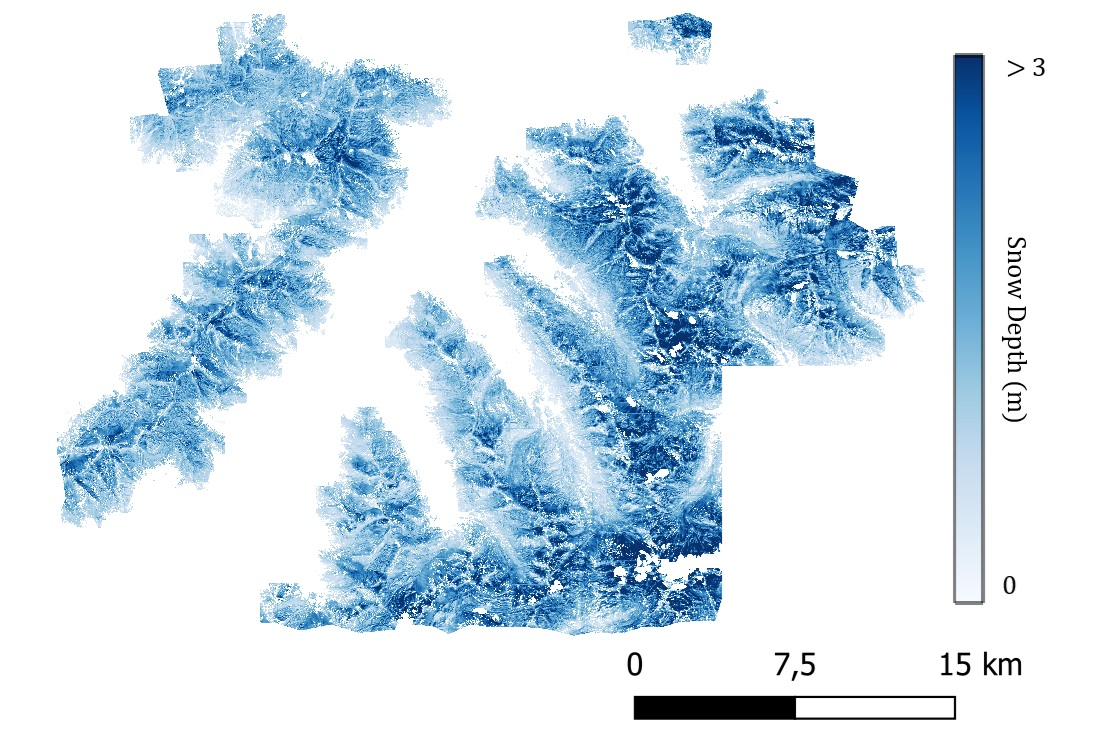
\includegraphics[width=0.8\textwidth]{snow_depth.jpg}
  \caption{Predicted snow depth for the Davos area (2017), where darker blue indicates greater snow accumulation.}
  \label{fig:predictionDavos2017}
\end{figure}

Figure \ref{fig:MAEDavos2017} depicts the differences between real and predicted snow depths across the Davos region, representing $y_i - \hat{y}_i$ for each grid cell, where $y_i$ is the observed snow depth and $\hat{y}_i$ is the predicted snow depth. The zero value (green color) represents areas where predictions closely matched observations, while the red and blue intensities indicate, respectively, the magnitude of underprediction and overprediction. The map's error distribution patterns align with the statistical analysis across multiple topographic variables. Of particular interest is the clear manifestation of elevation-dependent biases, where the transition from minimal errors in valley locations to pronounced overpredictions (blue) in higher alpine zones validates the assessment of elevation-related error patterns. However, detailed analysis reveals important nuances, such as the patterns observed in areas with very deep snow (2.9–4.0 m), where patches of red indicate localized underprediction. The map also highlights the relationship between slope and prediction accuracy, with notably stable predictions in areas of gentle terrain and increased error variability in steep zones, visually reinforcing the statistical findings.  
Furthermore, slopes facing south and southwest show consistently better prediction accuracy, as evidenced by the prevalence of green hues in these orientations. The influence of local topography is particularly well illustrated, as topographic depressions exhibit more pronounced prediction biases. These spatial patterns suggest that terrain-induced snow redistribution processes play a fundamental role in model performance.

%absolute differences between predicted and actual snow depths across the Davos region

\begin{figure}
  \centering
  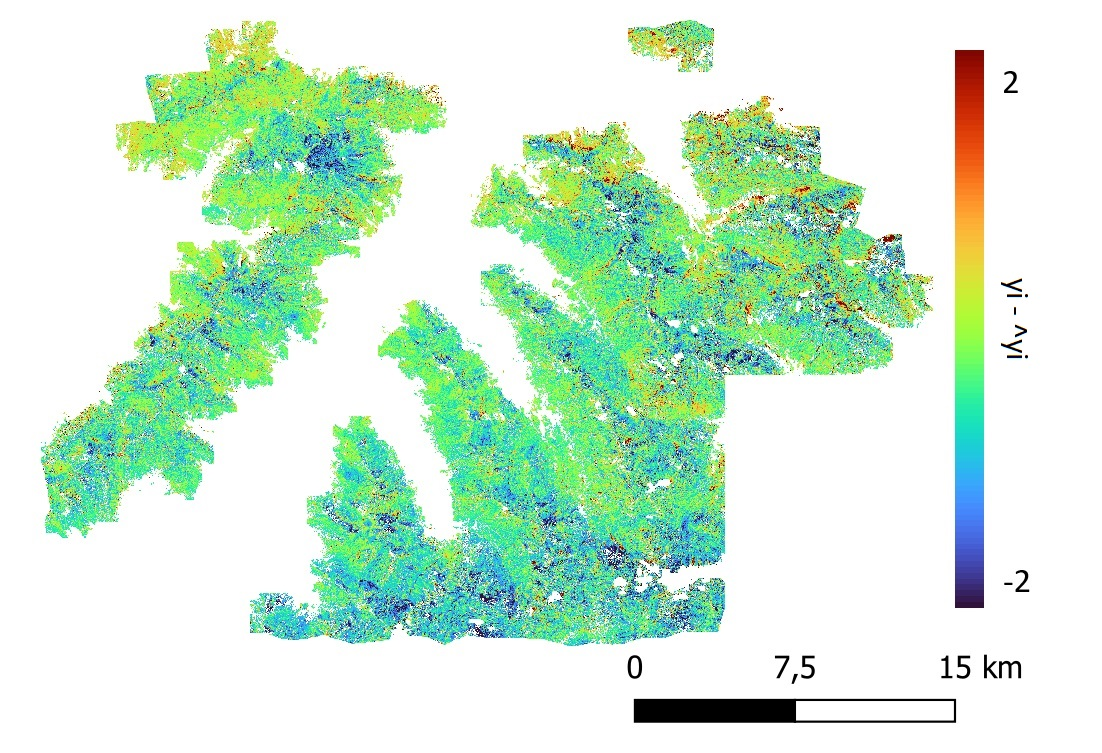
\includegraphics[width=0.8\textwidth]{snow prediction error.jpg}
  \caption{Differences between observed ($y_i$) and predicted ($\hat{y}_i$) snow depths across the Davos area (2017). Red color indicates underpredictions, blue color shows overpredictions, and green color represents accurate predictions.}
  \label{fig:MAEDavos2017}
\end{figure}

The spatial patterns observed in these maps reinforce our previous conclusions about the impact of topographical factors on snow depth measurement and prediction. The variability in error and uncertainty across the Davos area emphasizes the challenges in predicting snow depth in mountainous terrains. It also suggests that while our current model performs well in certain conditions, there's room for improvement in others, particularly in areas with steep slopes and high elevations.

Subsequently, we analyze the error distribution for snow depth to gain insights into the accuracy and reliability of our predictive model. Figure \ref{fig:Errors} shows the absolute error and the error ratio, defined as $Absolute\ error / HS$. The lowest error ratio is found at a snow depth of 2.52 m. In terms of absolute error, the minimum occurs at a snow depth of 1.72 m, with an MAE of 0.480 m, which is 8.5\% lower than the average error. This information could allow predictions to be accompanied by a confidence interval based on the error distribution.

\begin{figure*}[tb]
  \centering
  \begin{subfigure}{0.49\textwidth}
    \centering
    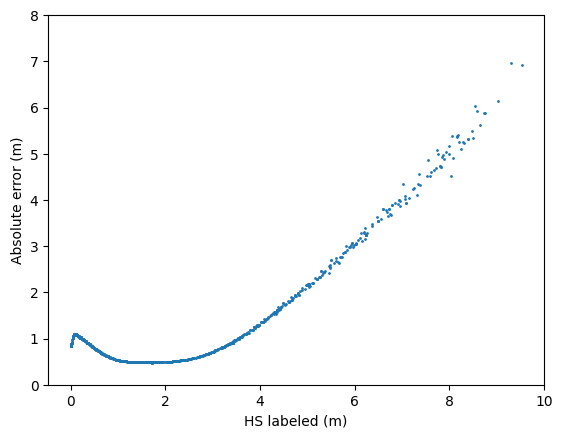
\includegraphics[width=\textwidth]{AbsError.png}
      \caption[Image 1]{}
      \label{fig:AbsError}
  \end{subfigure}
  \hfill                              %% no blank line here.
  \begin{subfigure}{0.49\textwidth}
    \centering
    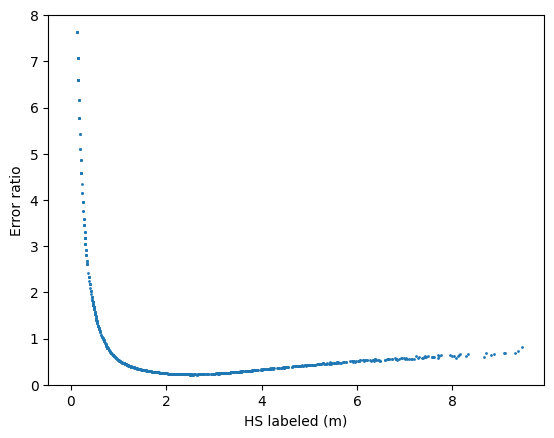
\includegraphics[width=\textwidth]{ErrorRatio.png}
      \caption[Image 2]{}
      \label{fig:ErrorRatio}
  \end{subfigure}
  \caption[Images]{Error distribution for snow depth (HS): (a) absolute error and (b) error ratio.}
  \label{fig:Errors}
\end{figure*}

When we examine the error ratio more closely, it becomes apparent that the model experiences a significant increase in the error ratio for predictions below 0.5 m. An interesting observation about the dataset is that snow depths under 0.5 m are exclusively found in a specific region with close to zero snow depth and predictions ranging from 0.5 to 1 m. In the training set, only 14\% of the samples have snow depths under 50 cm. This underscores the significance of representing features accurately, specifically the limited representation of low snow depth in this case. On the other hand, the absolute error reveals that predictions for greater snow depths tend to be less precise than those for shallower depths. As mentioned in the previous section, there is a tendency for underprediction in higher snow depths. This may indicate that not only is more data needed in lower snow depths, but also in higher ones. In our training set, only 9.7\% of the samples correspond to depths over 3 m and only 3.0\% over 4 m. Both effects together suggest that an effort should be put into creating a more balanced dataset in terms of snow depths.


\subsubsection{Comparative Analysis with other Snow Depth Estimation Methods}

The MAPunet approach for snow depth estimation offers distinct advantages over recent studies in terms of scale, complexity, and model performance. Geissler et al. \cite{Geissler2023} achieved remarkable accuracy (RMSE of 0.09 to 0.11 m at 1 m$^2$ resolution) in a small sub-alpine area (0.3 km$^2$) using a dense network of 16 measurement stations and LIDAR HS maps. Similarly, Revuelto et al. \cite{revuelto2020random} analyzed three sites totaling 1.03 km$^2$, employing a random forest algorithm at 1 m$^2$ resolution, which yielded MAE values between 0.80 and 1.13 m based on cross-validation results. However, the narrow range of conditions in these studies --primarily focused on sub-alpine environments and specific elevations-- limits their applicability to more diverse real-world settings. As noted by Revuelto et al. \cite{revuelto2020random}, ``\textit{random forests are not able to simulate snow depth distribution on sites not included in the training dataset}''. In contrast, MAPunet effectively addresses these challenges by operating across a much larger and diverse geographical area (369 km$^2$) in the Davos region, achieving a reasonable MAE of 0.62 m at a resolution of 5 m$^2$, despite dealing with sparse data and complex terrain.
% The range of conditions explored in these studies is relatively narrow and exhibits limited diversity. For example, Geissler’s research is focused on a sub-alpine environment with moderate slopes ranging from 11$^{\circ}$ to 25$^{\circ}$, while Revuelto’s sites are located at elevations between 2000 and 2800 m, with a maximum elevation variation of 300 m. 

%In consequence, these approaches, while valuable in controlled settings, face significant challenges when scaled to real-world applications where dense measurement networks and UAV flights are impractical. In fact, Revuelto states that "random forests are not able to simulate snow depth distribution on sites not included in the training dataset". In contrast, MAPunet directly addresses the challenges of real-world snow depth estimation by handling sparse data across a much larger and more diverse geographical area (369 km²) in the Davos region. Despite working with less dense measurements and more complex terrain, our model achieved a reasonable MAE of 0.525m with a resolution of 5 m$^2$}

Recent large-scale studies have also advanced snow monitoring through satellite-based methods and machine learning. For instance, Lievens et al. \cite{lievens2022sentinel} evaluated the Sentinel-1 mission for snow depth estimation across the European Alps from 2017 to 2019 at sub-kilometer resolutions (100 m, 500 m, and 1 km), reporting MAE ranges of 20\% to 30\% for depths between 1.5 and 3 m. Their performance degraded slightly at finer resolutions (100 m) and with very shallow or deep snowpacks, mirroring challenges encountered in our research. For their part, Dunmire et al. \cite{dunmire2024machine} applied XGBoost models to Sentinel-1 data, achieving an MAE of 0.18 m across 798 sites with over 50 coincident snow depth observations. However, the model faced difficulties estimating depths greater than 3 m, especially during peak snow conditions.

% Other recent large-scale studies have demonstrated significant progress in snow monitoring using both satellite-based methods and machine learning techniques. A notable example is the work by Lievens et al.\cite{lievens2022sentinel}, which evaluates the capability of the Sentinel-1 mission to estimate snow depth across the European Alps from 2017 to 2019 at sub-kilometer resolutions (100 m, 500 m, and 1 km). Their findings show that MAE ranges between 20\% and 30\% for snow depths between 1.5 and 3 m. However, performance slightly degrades at the finest resolution (100 m) and for very shallow or very deep snowpacks, which is similar to the challenges we encounter in our research.
% Another significant study is that of Dunmire et al.\cite{dunmire2024machine}, which applies machine learning models (XGBoost) to estimate snow depth using Sentinel-1 data. The MAE of the model is 0.18 m for 798 sites with over 50 coincident snow depth observations, excluding cases where measured snow depth was 0 m, having an MAE of 0.38 for times of peak snow depth. Dunmire’s model operates at a spatial resolution of 100 m, having the lowest relative error for in-situ snow depths between 1 and 3 m, but it faces challenges when estimating snow depths greater than 3 m.

In summary, MAPunet bridges the gap between highly detailed yet localized studies and large-scale satellite-based approaches. By offering a 5 m$^2$ resolution and significantly more spatial detail compared to other large-scale studies operating at 100 m to 1 km, MAPunet achieves a slightly higher MAE of 0.62 m. This trade-off between resolution and accuracy positions MAPunet as a practical solution for operational snow depth monitoring, addressing the need for greater spatial detail and extensive geographical coverage.

\subsubsection{Spatial and Temporal Generalization Capabilities}

The model appears to maintain some generalization capability across space and time, as suggested by the moderate increase in error when moving from validation (MAE: 0.525 m, RMSE: 0.634 m) to test (MAE: 0.62 m, RMSE: 0.80 m) sets, reflecting only an 18\% rise in MAE. This stability is favorable compared to studies like Revuelto et al. \cite{revuelto2020random}, which reported a 300\% error increase from training (MAE: 0.14-0.36 m) to test (MAE: 0.80--1.13 m) conditions. The more consistent performance of our model between the validation and test sets suggests that it has captured the relationships between topographic features and snow depth patterns, rather than overfitting to specific spatial patterns.

Spatially, our model has demonstrated effective generalization across a substantial area (369 km²) of complex alpine terrain, maintaining reasonable accuracy. The model's performance shows systematic patterns related to topographical features, performing better on gentle to moderate slopes at lower elevations and aspects ranging from 150° to 250°. This understanding of performance characteristics allows us to predict where the model will generalize well to new areas with similar topographical features.

For temporal generalization, while dynamic temporal variables enhance adaptability across the snow season, the study's temporal scope is currently limited, as the results are analyzed for only a single day. This constraint limits insights into how the framework performs over time. Two key challenges affect temporal performance: (1) model training has primarily used peak snow conditions, which limits accuracy during accumulation and melt phases; and (2) reliance on weather station data can hinder deployment in regions with sparse data coverage. Additionally, the training data distribution poses challenges for extreme snow depths, with only 14\% of the samples representing snow depths below 50 cm and 9.7\% above 3 m. As a result, uncertainty increases for shallow ($<$0.5 m) and deep snow conditions, leading to a tendency for underprediction at greater snow depths.

\section{Conclusions} \label{Sec:discussion}

%By adapting the U-Net architecture for pixel-wise regression, we have demonstrated its effectiveness in handling complex spatial data and producing high-quality results by generating accurate snow depth maps using geospatial and satellite imagery. Resolution also plays a crucial role in snow depth mapping: higher resolution leads to more complex terrain and, therefore, more complex snow accumulation patterns.
Regarding the research questions motivating this study, the following conclusions can be drawn.

1.- Can we develop an accurate, high-resolution (5 m) snow depth prediction model for the Davos region?
This manuscript introduces MAPunet, a U-Net based architecture specifically adapted for pixel-wise regression using a customized loss function. MAPunet effectively integrates various input features extracted from geospatial and satellite imagery to generate snow depth maps that retain the original input dimensions. The input maps are processed using MAPchete, a novel data augmentation and preprocessing tool designed to handle irregular maps, which is openly available for further research. Our experiments validate the model’s ability to manage complex spatial data and map snow depth at a 5 m resolution within the Davos area. 


2.- Which static and dynamic variables most influence snow depth predictions in this Alpine context? MAPunet's accuracy is achieved through the careful selection of the most informative variables from ten input features. The analysis identifies TPI as the most influential factor, followed by SCE. Other significant variables include aspect, DEM, and slope. Recognizing the importance of temporal dependencies in snow modeling, we developed three novel features --DEMStat, Voronoi, and ProbStat-- using data from meteorological stations. While DEMStat initially appeared less influential in the ablation study, this finding primarily reflects methodological challenges, especially given the sparse distribution of weather stations, which are concentrated in wind-sheltered, avalanche-prone areas at specific elevations. Finally, ProbStat demonstrated the best performance, achieving an MAE of 0.62 m and an RMSE of 0.80 m, confirming its effectiveness when high-quality data are available. Future research could explore combining ProbStat and DEMStat to enhance predictive accuracy by balancing altitude data with information from nearby stations.


3.- How does our model perform across various topographical features and snow conditions within Davos?
The model performs best in areas with moderate topographical characteristics, particularly at lower elevations and on south- and southwest-facing slopes. Performance deteriorates significantly at higher elevations, on steep slopes, and in topographic depressions. Regarding snow conditions, the FFD variable showed better performance when slopes align with the direction of minimum snow accumulation. These findings suggest that the model is most reliable in areas with moderate topographical characteristics and consistent snow accumulation patterns, while extreme terrain characteristics present the greatest challenges for accurate predictions.

Several avenues for further study are identified. First, exploring and comparing alternative models and architectural variations within the U-Net framework could lead to more effective snow depth mapping models. Second, increasing spatial resolution could improve the accuracy of hydrological models based on snow depth predictions. Third, incorporating additional dynamic input features, such as meteorological variables, could enhance our understanding of snow dynamics and improve the predictive power of our model. Fourth, gathering more comprehensive data on shallow and deep snow depths, including snow accumulation and melt phases, is crucial for refining our model and ensuring its robustness across diverse snow conditions and terrains. Finally, applying the proposed methodology to estimate snow depth in other regions by retraining the network with local data offers exciting opportunities, particularly in areas where high-quality reference data are available.

\section*{Acknowledgments}

This work was partially funded by the Spanish Ministry for Digital Transformation and Civil Service under grant TSI-10091-2023-4 and by the Asturian Government under research grant Severo Ochoa.

\section*{Data and code availability}

This study integrates publicly available data, derived products, and proprietary commercial code and data protected under a non-disclosure agreement (NDA). For information on data access and code availability, please contact the corresponding author.

\begin{thebibliography}{10}
\expandafter\ifx\csname url\endcsname\relax
  \def\url#1{\texttt{#1}}\fi
\expandafter\ifx\csname urlprefix\endcsname\relax\def\urlprefix{URL }\fi
\expandafter\ifx\csname href\endcsname\relax
  \def\href#1#2{#2} \def\path#1{#1}\fi

\bibitem{xu2013snow}
L.~Xu, P.~Dirmeyer, {Snow--atmosphere coupling strength. Part II: Albedo effect versus hydrological effect}, Journal of Hydrometeorology 14~(2) (2013) 404--418.

\bibitem{fenrg.2024}
Y.~Frischholz, U.~Schilt, V.~Sharma, A.~Kahl, S.~Strebel, D.~Anderegg, J.~Rohrer, M.~Lehning, {Confirmation of the power gain for solar photovoltaic systems in alpine areas and across scales}, Frontiers in Energy Research 12 (2024).

\bibitem{vonRtte2021}
F.~von R\"{u}tte, A.~Kahl, J.~Rohrer, M.~Lehning, {How Forward‐Scattering Snow and Terrain Change the Alpine Radiation Balance With Application to Solar Panels}, Journal of Geophysical Research: Atmospheres 126~(15) (2021).

\bibitem{wegawSuperResolutionSnow}
T.~James, {S}uper-{R}esolution {S}now {H}eight: {D}eep {L}earning {S}olutions for {S}olar {P}ower - {W}egaw --- wegaw.com, \url{https://wegaw.com/super-resolution-snow-height-deep-learning-solutions-for-solar-power/}, [Accessed 2024-10-25] (2023).

\bibitem{dewalle2008principles}
D.~R. DeWalle, A.~Rango, Principles of snow hydrology, Cambridge University Press, 2008.

\bibitem{Kahl2019}
A.~Kahl, J.~Dujardin, M.~Lehning, {The bright side of PV production in snow-covered mountains}, Proceedings of the National Academy of Sciences 116~(4) (2019) 1162--1167.

\bibitem{Dujardin2022}
J.~Dujardin, M.~Schillinger, A.~Kahl, J.~Savelsberg, I.~Schlecht, R.~Lordan-Perret, Optimized market value of alpine solar photovoltaic installations, Renewable Energy 186 (2022) 878–888.

\bibitem{liu2019retrieval}
J.~Liu, Y.~Zhang, X.~Cheng, Y.~Hu, {Retrieval of snow depth over Arctic sea ice using a deep neural network}, Remote Sensing 11~(23) (2019) 2864.

\bibitem{Tedesco2010}
M.~Tedesco, P.~S. Narvekar, {Assessment of the NASA AMSR-E SWE Product}, IEEE Journal of Selected Topics in Applied Earth Observations and Remote Sensing 3~(1) (2010) 141–159.

\bibitem{Tong2010}
J.~Tong, S.~J. Déry, P.~L. Jackson, C.~Derksen, {Testing snow water equivalent retrieval algorithms for passive microwave remote sensing in an alpine watershed of western Canada}, Canadian Journal of Remote Sensing 36~(sup1) (2010) S74–S86.

\bibitem{Smith2018}
T.~Smith, B.~Bookhagen, {Changes in seasonal snow water equivalent distribution in High Mountain Asia (1987 to 2009)}, Science Advances 4~(1) (2018).

\bibitem{revuelto2021intercomparison}
J.~Revuelto, E.~Alonso-Gonzalez, I.~Vidaller-Gayan, E.~Lacroix, E.~Izagirre, G.~Rodríguez-López, J.~I. López-Moreno, {Intercomparison of UAV platforms for mapping snow depth distribution in complex alpine terrain}, Cold Regions Science and Technology 190 (2021) 103344.

\bibitem{deems2013lidar}
J.~S. Deems, T.~H. Painter, D.~C. Finnegan, Lidar measurement of snow depth: a review, Journal of Glaciology 59~(215) (2013) 467--479.

\bibitem{buhler2016mapping}
Y.~Bühler, M.~S. Adams, R.~Bösch, A.~Stoffel, {Mapping snow depth in alpine terrain with unmanned aerial systems (UASs): potential and limitations}, The Cryosphere 10~(3) (2016) 1075--1088.

\bibitem{wulf2020high}
H.~Wulf, B.~Sassik, G.~Milani, R.~Leiterer, High-resolution snow depth monitoring for entire mountain ranges, in: 7th Swiss Conference on Data Science, IEEE, 2020, pp. 1--4.

\bibitem{cartwright2022machine}
K.~Cartwright, C.~Mahoney, C.~Hopkinson, {Machine learning based imputation of mountain snowpack depth within an operational Lidar sampling framework in Southwest Alberta}, Canadian Journal of Remote Sensing 48~(1) (2022) 107--125.

\bibitem{Dharmadasa2023}
V.~Dharmadasa, C.~Kinnard, M.~Bara\"er, {Topographic and vegetation controls of the spatial distribution of snow depth in agro-forested environments by UAV lidar}, The Cryosphere 17~(3) (2023) 1225--1246.

\bibitem{Dharmadasa2024}
V.~Dharmadasa, C.~Kinnard, M.~Bara{\"e}r, {A new interpolation method to resolve under-sampling of UAV-lidar snow depth observations in coniferous forests}, Cold Regions Science and Technology 220 (2024) 104134.

\bibitem{winstral2002spatial}
A.~Winstral, K.~Elder, R.~E. Davis, Spatial snow modeling of wind-redistributed snow using terrain-based parameters, Journal of Hydrometeorology 3~(5) (2002) 524--538.

\bibitem{hu2021snow}
Y.~Hu, T.~Che, L.~Dai, L.~Xiao, {Snow depth fusion based on machine learning methods for the Northern Hemisphere}, Remote Sensing 13~(7) (2021) 1250.

\bibitem{wang2020estimating}
J.~Wang, Q.~Yuan, H.~Shen, T.~Liu, T.~Li, L.~Yue, X.~Shi, L.~Zhang, {Estimating snow depth by combining satellite data and ground-based observations over Alaska: A deep learning approach}, Journal of Hydrology 585 (2020) 124828.

\bibitem{meyal2020automated}
A.~Y. Meyal, R.~Versteeg, E.~Alper, D.~Johnson, A.~Rodzianko, M.~Franklin, H.~Wainwright, {Automated cloud based long short-term memory neural network based SWE prediction}, Frontiers in Water 2 (2020) 574917.

\bibitem{xing2022estimation}
D.~Xing, J.~Hou, C.~Huang, W.~Zhang, {Estimation of Snow Depth from AMSR2 and MODIS Data based on Deep Residual Learning Network}, Remote Sensing 14~(20) (2022) 5089.

\bibitem{Geissler2023}
J.~Geissler, L.~Rathmann, M.~Weiler, {Combining Daily Sensor Observations and Spatial LiDAR Data for Mapping Snow Water Equivalent in a Sub‐Alpine Forest}, Water Resources Research 59~(9) (2023).

\bibitem{revuelto2020random}
J.~Revuelto, P.~Billecocq, F.~Tuzet, B.~Cluzet, M.~Lamare, F.~Larue, M.~Dumont, Random forests as a tool to understand the snow depth distribution and its evolution in mountain areas, Hydrological Processes 34~(26) (2020) 5384--5401.

\bibitem{daudt2023snow}
R.~C. Daudt, H.~Wulf, E.~D. Hafner, Y.~Bühler, K.~Schindler, J.~D. Wegner, Snow depth estimation at country-scale with high spatial and temporal resolution, ISPRS Journal of Photogrammetry and Remote Sensing 197 (2023) 105--121.

\bibitem{eberhard2021intercomparison}
L.~A. Eberhard, P.~Sirguey, A.~Miller, M.~Marty, K.~Schindler, A.~Stoffel, Y.~Bühler, Intercomparison of photogrammetric platforms for spatially continuous snow depth mapping, The Cryosphere 15~(1) (2021) 69--94.

\bibitem{dunmire2024machine}
D.~Dunmire, H.~Lievens, L.~Boeykens, G.~J. De~Lannoy, {A machine learning approach for estimating snow depth across the European Alps from Sentinel-1 imagery}, Remote Sensing of Environment 314 (2024) 114369.

\bibitem{broxton2024improving}
P.~Broxton, M.~R. Ehsani, A.~Behrangi, {Improving mountain snowpack estimation using machine learning with Sentinel-1, the Airborne Snow Observatory, and University of Arizona snowpack data}, Earth and Space Science 11~(3) (2024) e2023EA002964.

\bibitem{ronneberger2015u}
O.~Ronneberger, P.~Fischer, T.~Brox, {U-net: Convolutional networks for biomedical image segmentation}, in: 18th International Conference on Medical Image Computing and Computer-assisted Intervention, part III 18, 2015, pp. 234--241.

\bibitem{YAO2018}
W.~Yao, Z.~Zeng, C.~Lian, H.~Tang, {Pixel-wise regression using U-Net and its application on pansharpening}, Neurocomputing 312 (2018) 364--371.

\bibitem{TACCARI2022}
M.~L. Taccari, J.~Nuttall, X.~Chen, H.~Wang, B.~Minnema, P.~K. Jimack, {Attention U-Net as a surrogate model for groundwater prediction}, Advances in Water Resources 163 (2022) 104169.

\bibitem{Yin2022}
M.~Yin, P.~Wang, C.~Ni, W.~Hao, {Cloud and snow detection of remote sensing images based on improved Unet3+}, Scientific Reports 12~(1) (2022).

\bibitem{Wang2022}
Y.~Wang, J.~Su, X.~Zhai, F.~Meng, C.~Liu, {Snow Coverage Mapping by Learning from Sentinel-2 Satellite Multispectral Images via Machine Learning Algorithms}, Remote Sensing 14~(3) (2022) 782.

\bibitem{Ma2023}
J.~Ma, H.~Shen, Y.~Cai, T.~Zhang, J.~Su, W.-H. Chen, J.~Li, {UCTNet with Dual-Flow Architecture: Snow Coverage Mapping with Sentinel-2 Satellite Imagery}, Remote Sensing 15~(17) (2023) 4213.

\bibitem{zhu2021downscaling}
L.~Zhu, Y.~Zhang, J.~Wang, W.~Tian, Q.~Liu, G.~Ma, X.~Kan, Y.~Chu, Downscaling snow depth mapping by fusion of microwave and optical remote-sensing data based on deep learning, Remote Sensing 13~(4) (2021) 584.

\bibitem{zhong2021impacts}
X.-Y. Zhong, T.~Zhang, H.~Su, X.-X. Xiao, S.-F. Wang, Y.-T. Hu, H.-J. Wang, L.~Zheng, W.~Zhang, M.~Xu, et~al., {Impacts of landscape and climatic factors on snow cover in the Altai Mountains, China}, Advances in Climate Change Research 12~(1) (2021) 95--107.

\bibitem{scott2015multivariate}
D.~W. Scott, Multivariate density estimation: theory, practice, and visualization, John Wiley \& Sons, 2015.

\bibitem{lindsay2014whitebox}
J.~Lindsay, {The whitebox geospatial analysis tools project and open-access GIS}, in: 22nd Annual Conference on GIS Research UK, 2014, pp. 16--18.

\bibitem{newman2018evaluating}
D.~Newman, J.~Lindsay, J.~Cockburn, Evaluating metrics of local topographic position for multiscale geomorphometric analysis, Geomorphology 312 (2018) 40--50.

\bibitem{grizonnet2017operational}
M.~Grizonnet, {An operational snow cover product from Sentinel-2 and Landsat-8 data for mountain regions}, in: La montagne, territoire d'innovation, 2017.

\bibitem{Gascoin2019}
S.~Gascoin, M.~Grizonnet, M.~Bouchet, G.~Salgues, O.~Hagolle, {Theia Snow collection: high-resolution operational snow cover maps from Sentinel-2 and Landsat-8 data}, Earth System Science Data 11~(2) (2019) 493--514.

\bibitem{Main-Knorn2017}
M.~Main-Knorn, B.~Pflug, J.~Louis, V.~Debaecker, U.~M{\"u}ller-Wilm, F.~Gascon, {Sen2Cor for Sentinel-2}, in: Image and signal processing for remote sensing XXIII, Vol. 10427, 2017, pp. 37--48.

\bibitem{Grunewald2014}
T.~Gr\"unewald, Y.~B\"uhler, M.~Lehning, Elevation dependency of mountain snow depth, The Cryosphere 8~(6) (2014) 2381--2394.

\bibitem{kramer2016scikit}
O.~Kramer, O.~Kramer, Scikit-learn, Machine Learning for Evolution Strategies (2016) 45--53.

\bibitem{lang2023}
N.~Lang, W.~Jetz, K.~Schindler, J.~D. Wegner, {A high-resolution canopy height model of the Earth}, Nature Ecology \& Evolution 7~(11) (2023) 1778–1789.

\bibitem{collobert2011torch7}
R.~Collobert, K.~Kavukcuoglu, C.~Farabet, {Torch7: A matlab-like environment for machine learning}, in: BigLearn, NIPS workshop, 2011, pp. 1--6.

\bibitem{RichDEM}
R.~Barnes, \href{http://github.com/r-barnes/richdem}{{RichDEM: Terrain Analysis Software}}, [Accessed 2024-10-25] (2016).
\newline\urlprefix\url{http://github.com/r-barnes/richdem}

\bibitem{Rasterio}
S.~Gillies, et~al., \href{https://github.com/mapbox/rasterio}{{Rasterio: geospatial raster I/O for Python programmers}}, [Accessed 2024-10-25] (2013).
\newline\urlprefix\url{https://github.com/mapbox/rasterio}

\bibitem{GDAL}
{GDAL/OGR contributors}, \href{https://gdal.org}{{GDAL/OGR} Geospatial Data Abstraction software Library}, Open Source Geospatial Foundation (2024).
\newblock \href {https://doi.org/10.5281/zenodo.5884351} {\path{doi:10.5281/zenodo.5884351}}.
\newline\urlprefix\url{https://gdal.org}

\bibitem{QGISsoftware}
Q.~D. Team, {QGIS Geographic Information System}, \url{https://www.qgis.org}, [Accessed 2024-10-25].

\bibitem{Bhler2015}
Y.~B\"uhler, M.~Marty, L.~Egli, J.~Veitinger, T.~Jonas, P.~Thee, C.~Ginzler, Snow depth mapping in high-alpine catchments using digital photogrammetry, The Cryosphere 9~(1) (2015) 229–243.

\bibitem{Buhler2023}
Y.~B\"{u}hler, A.~Stoffel, L.~Eberhard, L.~B\"{u}hrle, {Fotogrammetrische Schneeh\"{o}henkartierung aus Drohnen-, Flugzeug- und Satellitenbildern}, in: Neue Fernerkundungstechnologien f\"{u}r die Umweltforschung und Praxis, 2023.

\bibitem{Buhrle2023}
L.~J. B{\"u}hrle, M.~Marty, L.~A. Eberhard, A.~Stoffel, E.~D. Hafner, Y.~B{\"u}hler, Spatially continuous snow depth mapping by aeroplane photogrammetry for annual peak of winter from 2017 to 2021 in open areas, The Cryosphere 17~(8) (2023) 3383--3408.

\bibitem{kiefer1952stochastic}
J.~Kiefer, J.~Wolfowitz, Stochastic estimation of the maximum of a regression function, The Annals of Mathematical Statistics (1952) 462--466.

\bibitem{kingma2014adam}
D.~P. Kingma, J.~Ba, {Adam: A method for stochastic optimization}, arXiv preprint arXiv:1412.6980 (2014).

\bibitem{Branch99}
M.~A. Branch, T.~F. Coleman, Y.~Li, {A Subspace, Interior, and Conjugate Gradient Method for Large-Scale Bound-Constrained Minimization Problems}, SIAM Journal on Scientific Computing 21~(1) (1999) 1--23.

\bibitem{lievens2022sentinel}
H.~Lievens, I.~Brangers, H.-P. Marshall, T.~Jonas, M.~Olefs, G.~De~Lannoy, {Sentinel-1 snow depth retrieval at sub-kilometer resolution over the European Alps}, The Cryosphere 16~(1) (2022) 159--177.

\end{thebibliography}

\end{document}